\section{Smart Grapple control stack}

This section describes the software architecture and control modules that enable autonomous and manual operation of the Smart Grapple system. The control stack integrates state estimation using an Extended Kalman Filter that fuses IMU and DVL sensor data for position and velocity estimation, thruster control allocation for six-degree-of-freedom maneuvering, and joint control for the eight SensoJoint actuators via EtherCAT communication within the ROS~2 framework. A hierarchical state machine orchestrates the complete operation cycle through deploying, planning, tracking, visual servoing, grasping, and recovery phases, with provisions for error handling and seamless transitions between autonomous and manual control modes through dedicated graphical user interfaces.


\subsection{Smart Grapple State Estimation}
The goal of state estimation is to compute the approximate position and velocity of the \gls{usg}. This information is required for trajectory tracking during locomotion of the robot, as described in Section~\ref{sec:trackingState}. The proposed approach leverages an \gls{ekf} on the measured sensor data to achieve state estimation.

\textbf{Sensor fusion.}
Two types of sensors are used as data sources for state estimation: an \gls{imu} and a \gls{dvl}. The \gls{imu} provides measurements of linear acceleration and angular velocity, while the \gls{dvl} provides measurements of linear and angular velocity and altitude of the vehicle relative to the seabed. In order to increase the precision of state estimation, the \gls{imu} and \gls{dvl} measurements are fused together via the \gls{ekf} \cite{10.5555/897831}.

\begin{figure}[ht]
	\centering
	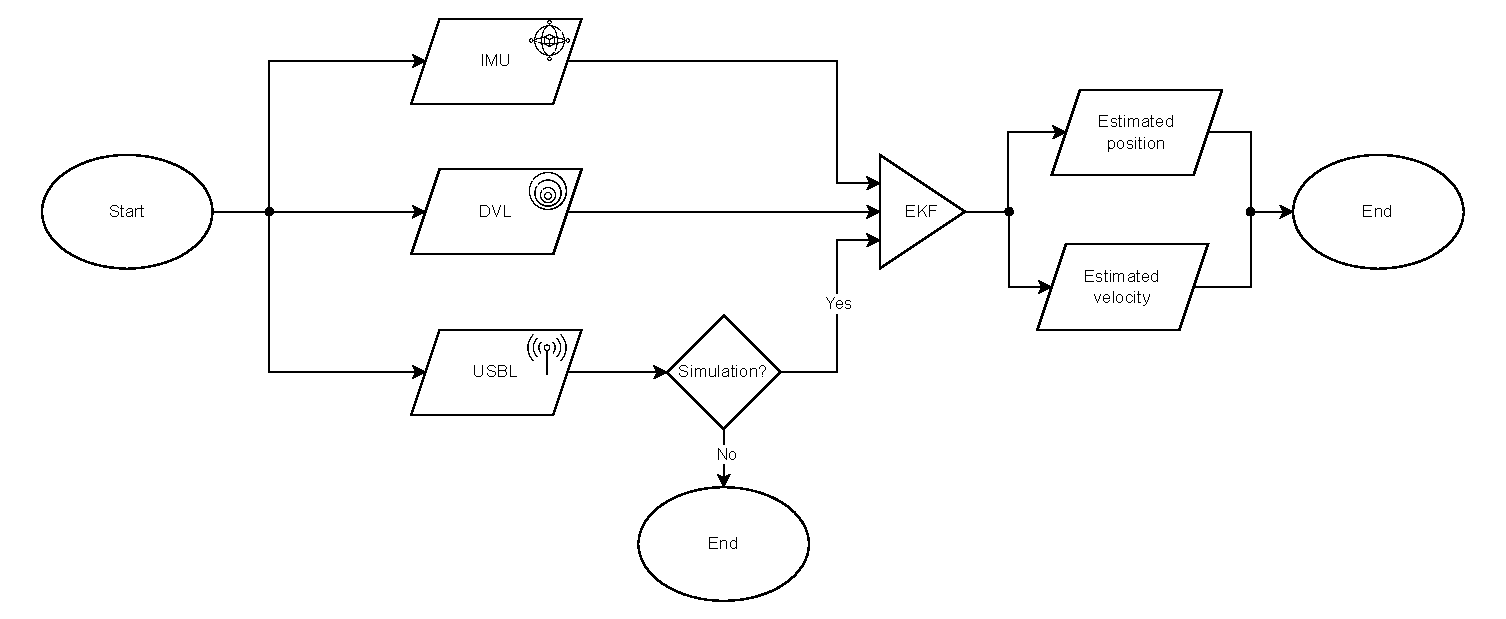
\includegraphics[width=\textwidth]{img/state_estimation_flowchart.drawio.pdf}
	\caption{Information flow of the state estimation}
	\label{fig:stateEstimationFlowchart}
\end{figure}

\textbf{Implementation.}
The \textit{robot\_localization} package, developed by Charles River Analytics, is used to implement the \gls{ekf} \cite{MooreStouchKeneralizedEkf2014}. It is an open-source package that provides a basic framework for localization tasks that can be easily adapted to different robotic systems such as the \gls{usg}. The main benefits of this package are:
\begin{itemize}
    \item Supports ROS 2 out-of-the-box,
    \item Handles an unlimited number of inputs from multiple sensor types,
    \item Allows 3D localization,
    \item Provides higher control over the sensor data and how it impacts the estimation.
\end{itemize}

\textbf{Simulation.}
The state estimation module is part of the digital twin. The data sources for sensor fusion in simulation are slightly different as they also include \gls{gnss} measurements. These measurements are used to emulate a \gls{usbl} acoustic positioning system, which will be added to the \gls{usg} hardware in the future. For more details on the digital twin, refer to Section~\ref{sec:sim}.

\subsection{Smart Grapple Control Allocation}

This section describes the control allocation system that distributes commanded wrenches across the eight thrusters mounted on the \gls{usg}. The allocation matrix is derived from the geometric configuration of the thrusters, mapping individual thrust commands to the resulting six-degree-of-freedom wrench at the center of mass. To handle the 5~kW power constraint shared among all thrusters, a quadratic programming formulation with a percentage phase-back post-processing strategy is employed, which maintains real-time computational feasibility (average runtime of 18~ms) while achieving tracking performance within 15.6\% of the optimal nonlinear solution.


\subsubsection{Thruster Positions on the Hardware}

\begin{figure}[!h]
    \centering
    %----------------------------------------------------------
    \begin{subfigure}[t]{0.48\textwidth}
        \centering
        % Crop left, bottom, right, top (adjust as needed)
        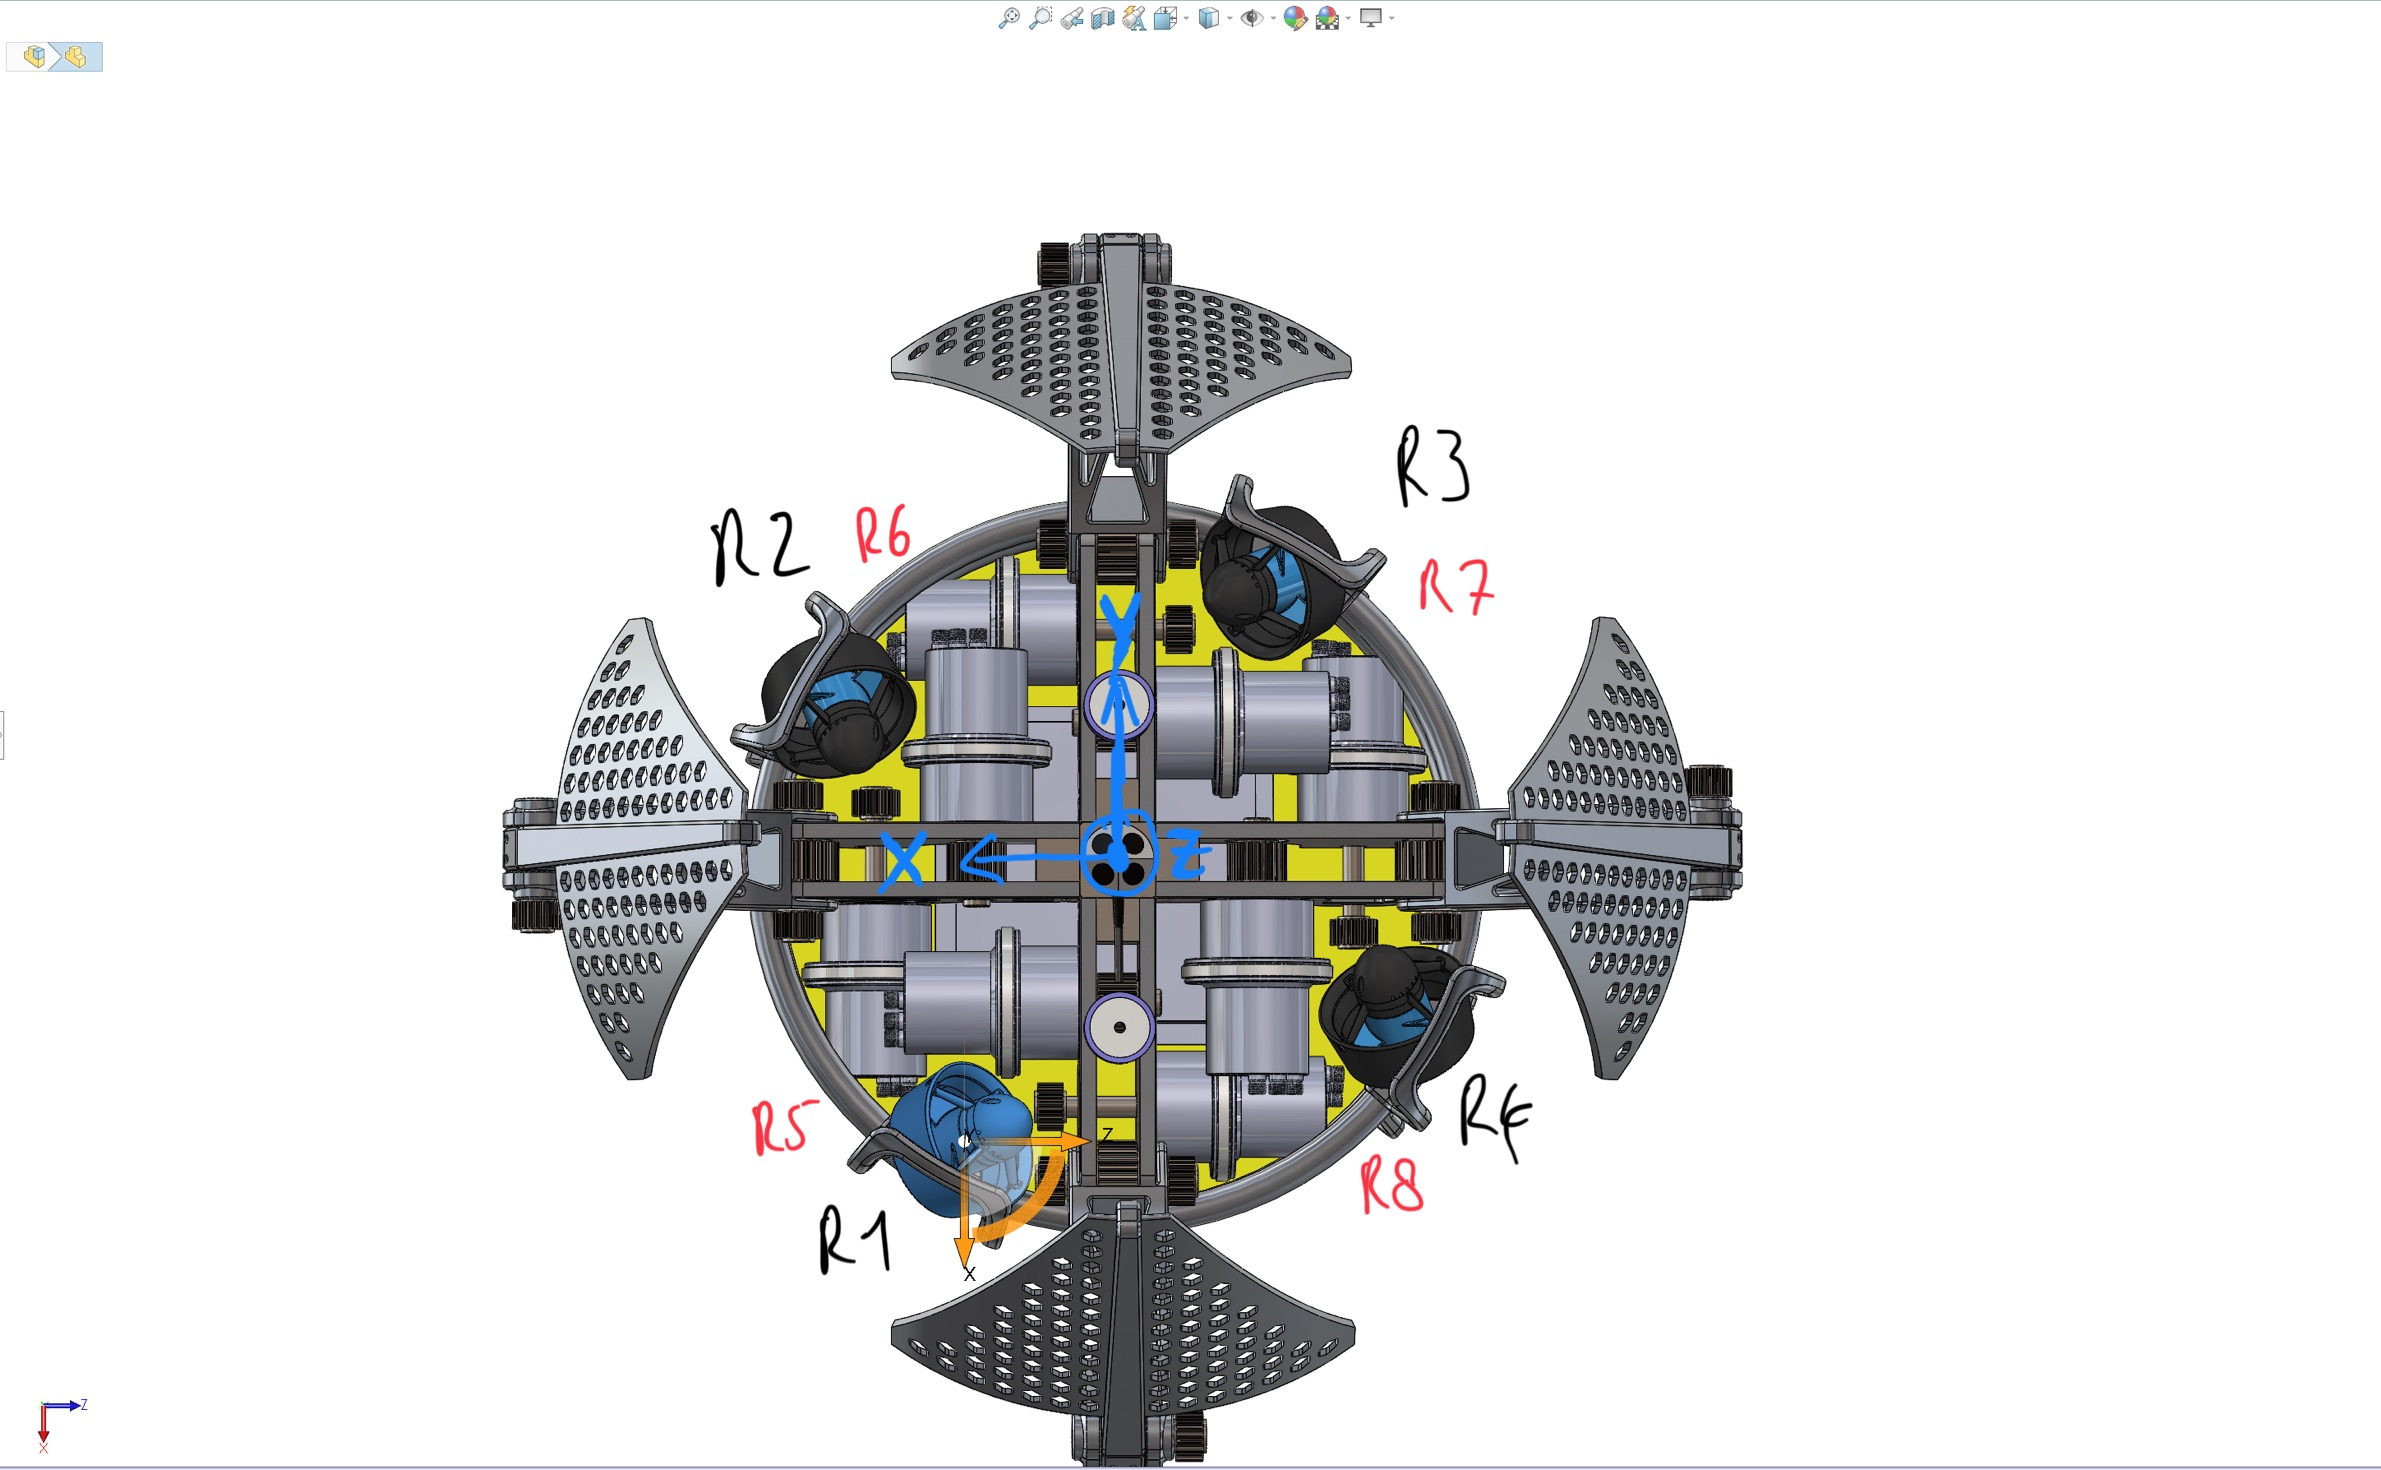
\includegraphics[width=\textwidth, trim={4cm 2cm 4cm 4cm}, clip]{img/bottom_view_thrusters.jpeg}
        \caption{Bottom view (looking along $-\!Z_{\mathrm{ref}}$). Thrusters R1–R4 shown in \textcolor{black}{black} (visible) and occluded units in \textcolor{red}{red}.}
        \label{fig:thrusters_bottom}
    \end{subfigure}
    \hfill
    %----------------------------------------------------------
    \begin{subfigure}[t]{0.48\textwidth}
        \centering
        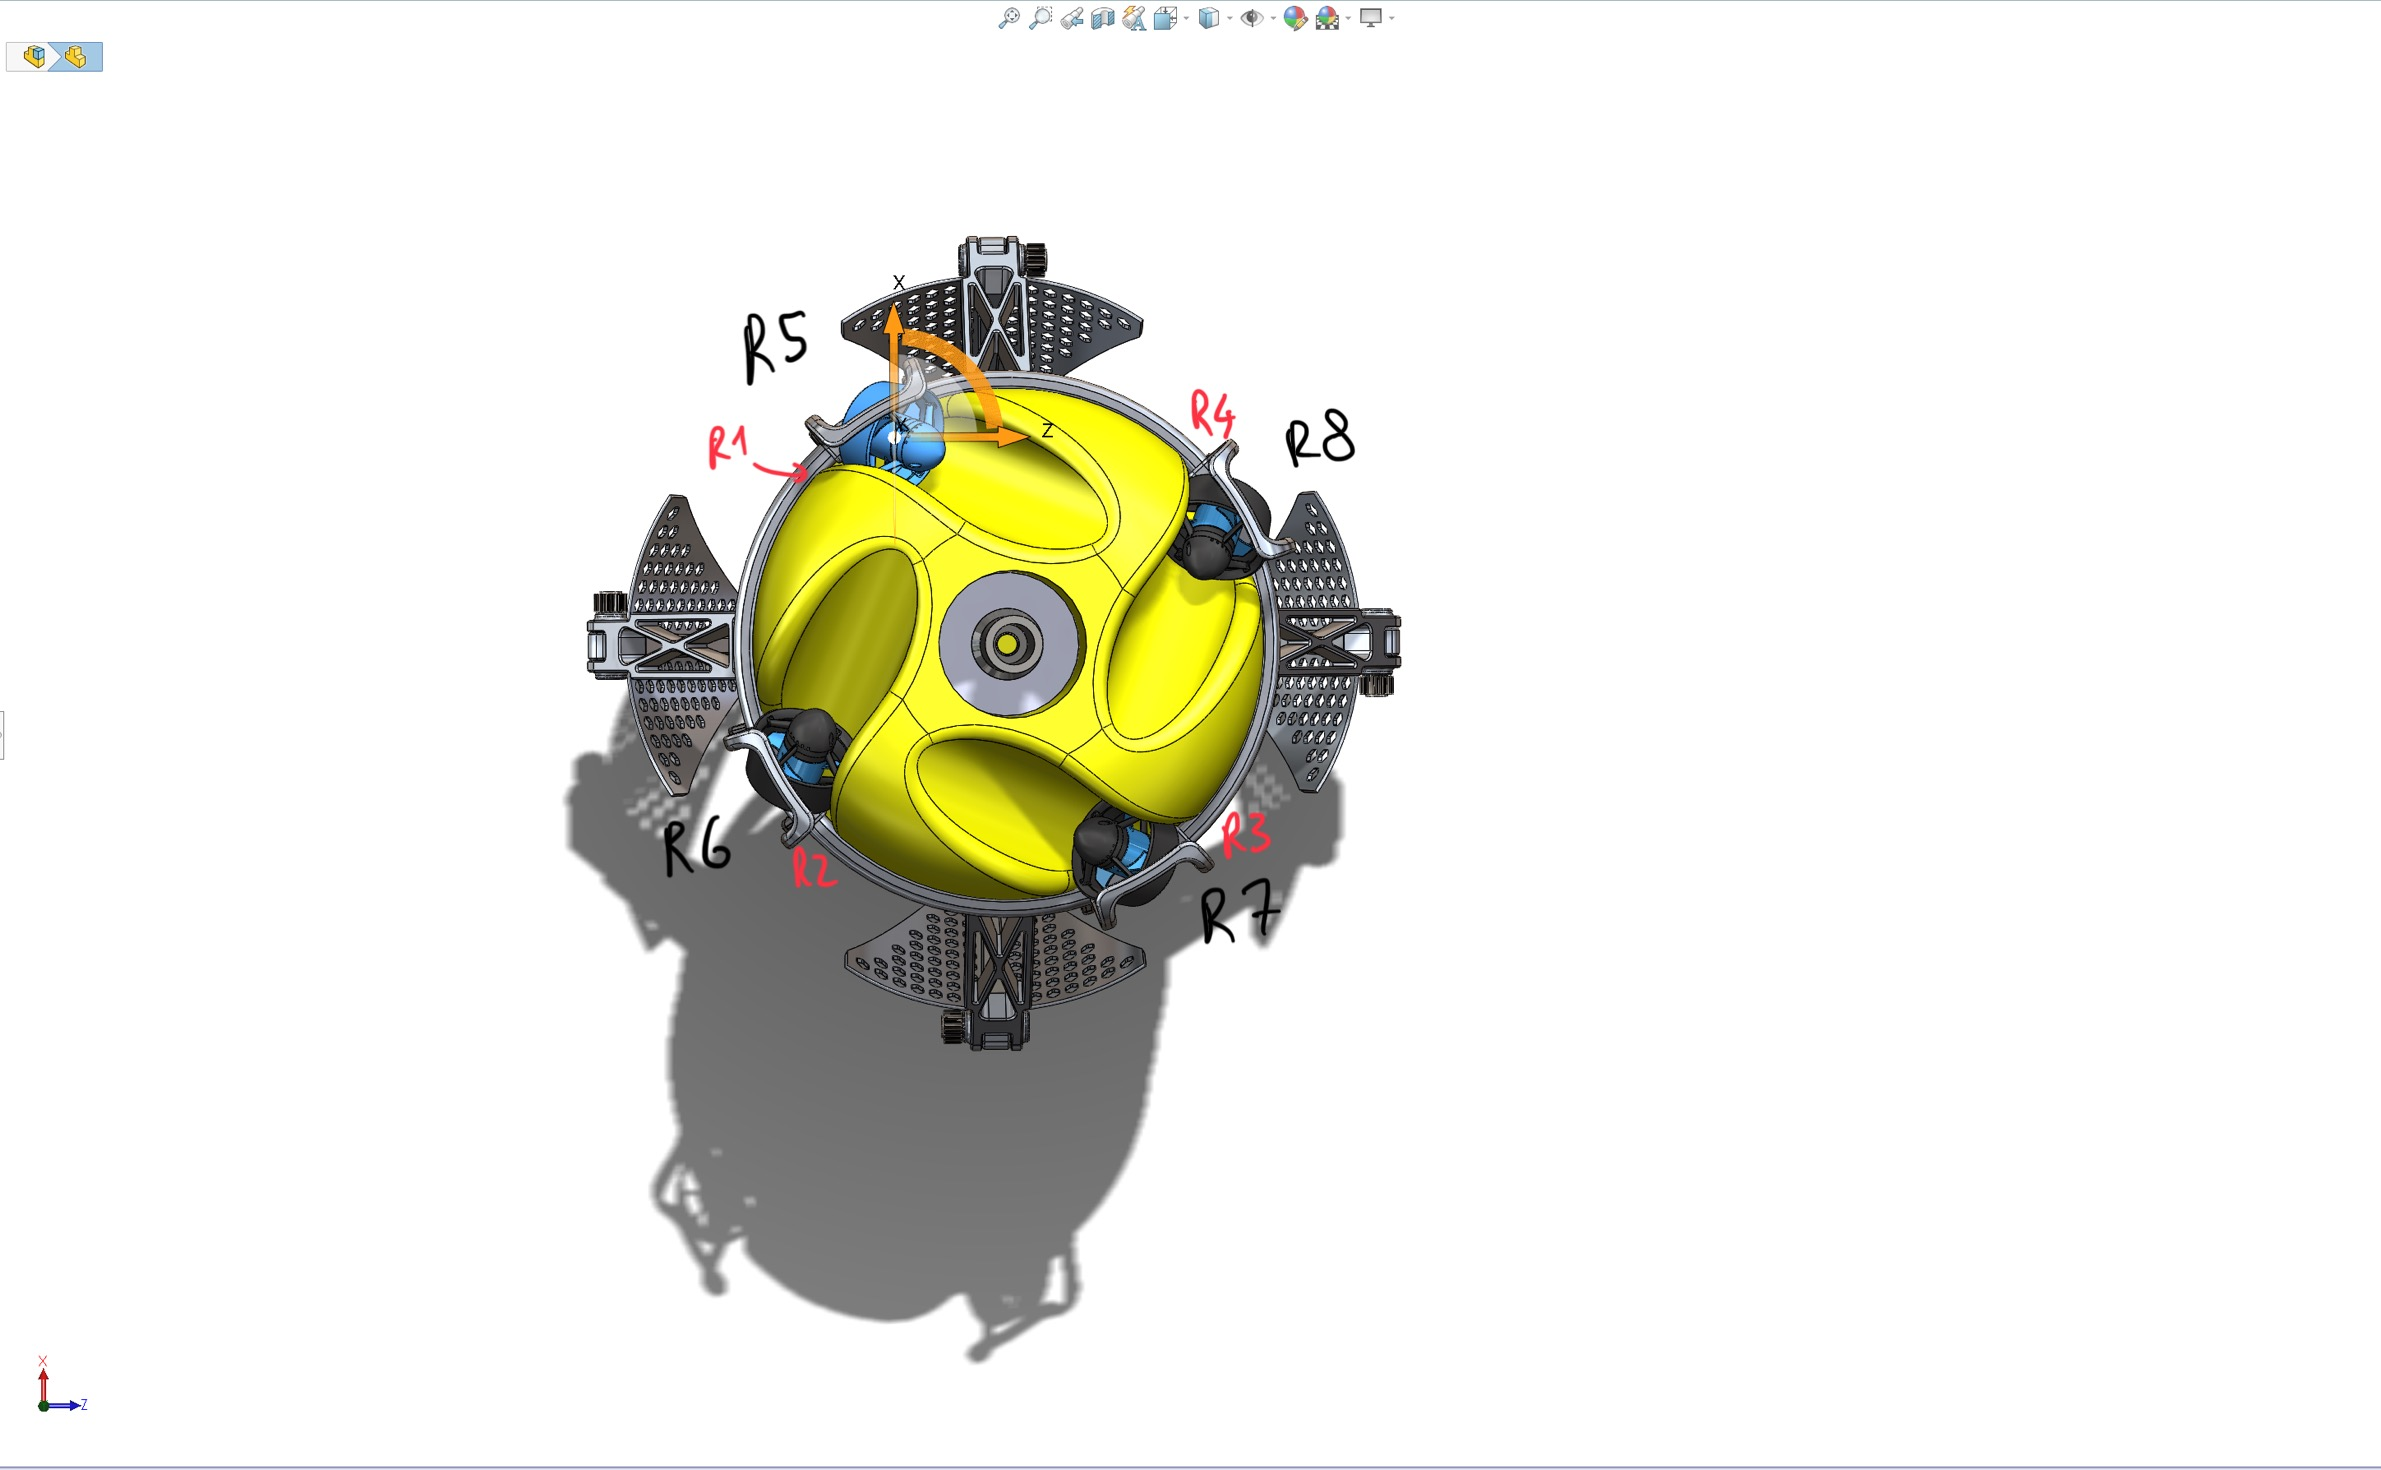
\includegraphics[width=\textwidth, trim={15cm 14cm 15cm 8cm}, clip]{img/top_view_thrusters.jpeg}
        \caption{Top view (looking along $+\!Z_{\mathrm{ref}}$). Thrusters R5–R8 shown in \textcolor{black}{black} (visible) and occluded units in \textcolor{red}{red}.}
        \label{fig:thrusters_top}
    \end{subfigure}
    %----------------------------------------------------------
    \caption{Thruster layout of the \gls{usg} platform in the reference frame $\mathcal{F}_{\mathrm{ref}}$ \textcolor{blue}{blue} \ian{in (a)}.
    \bds{It is not clear to me what "blue" refers to here}
    Subfigure~\subref{fig:thrusters_bottom} depicts the bottom assembly (R1–R4), and Subfigure~\subref{fig:thrusters_top} the top assembly (R5–R8).
    Color coding: \textcolor{black}{black} = visible in the current viewpoint; \textcolor{red}{red} = occluded.}
    \label{fig:thruster_overview}
\end{figure}
\begin{figure}[h!]
    \centering
    % Five rotated images with minimal whitespace
    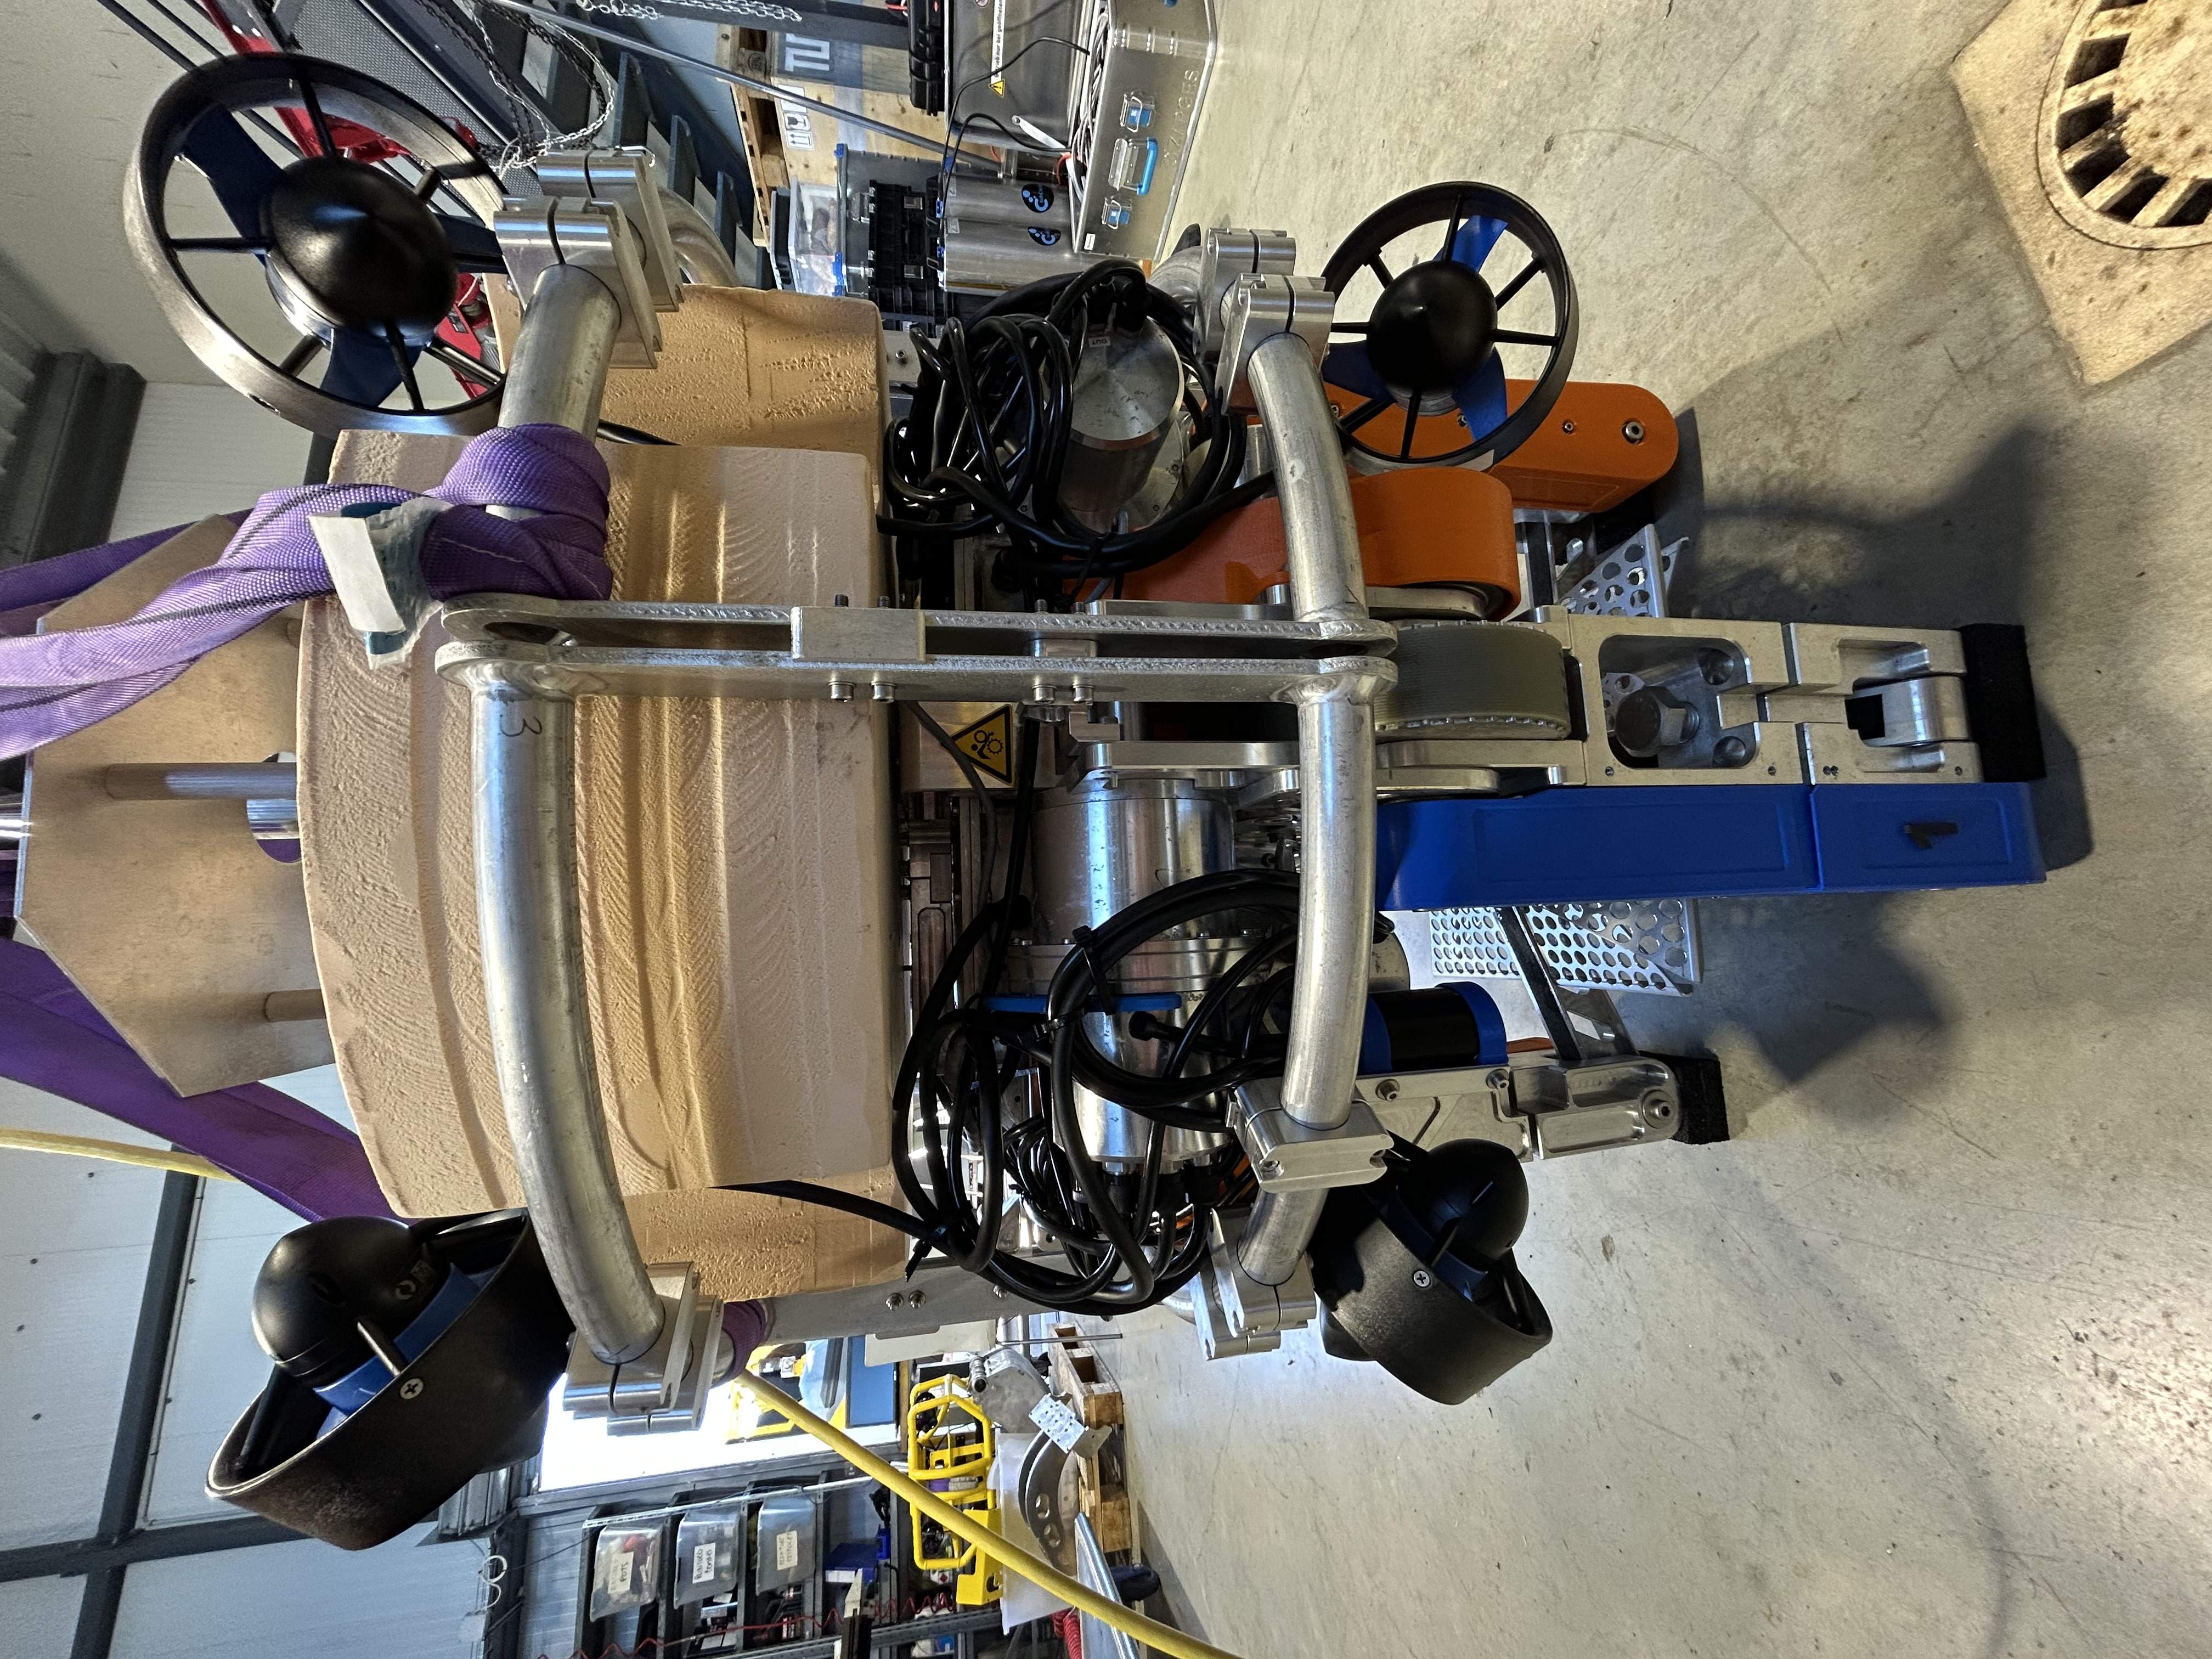
\includegraphics[width=0.25\textwidth, angle=270, origin=c]{img/grapple_thrusters_1.jpeg}\hspace{2pt}%
    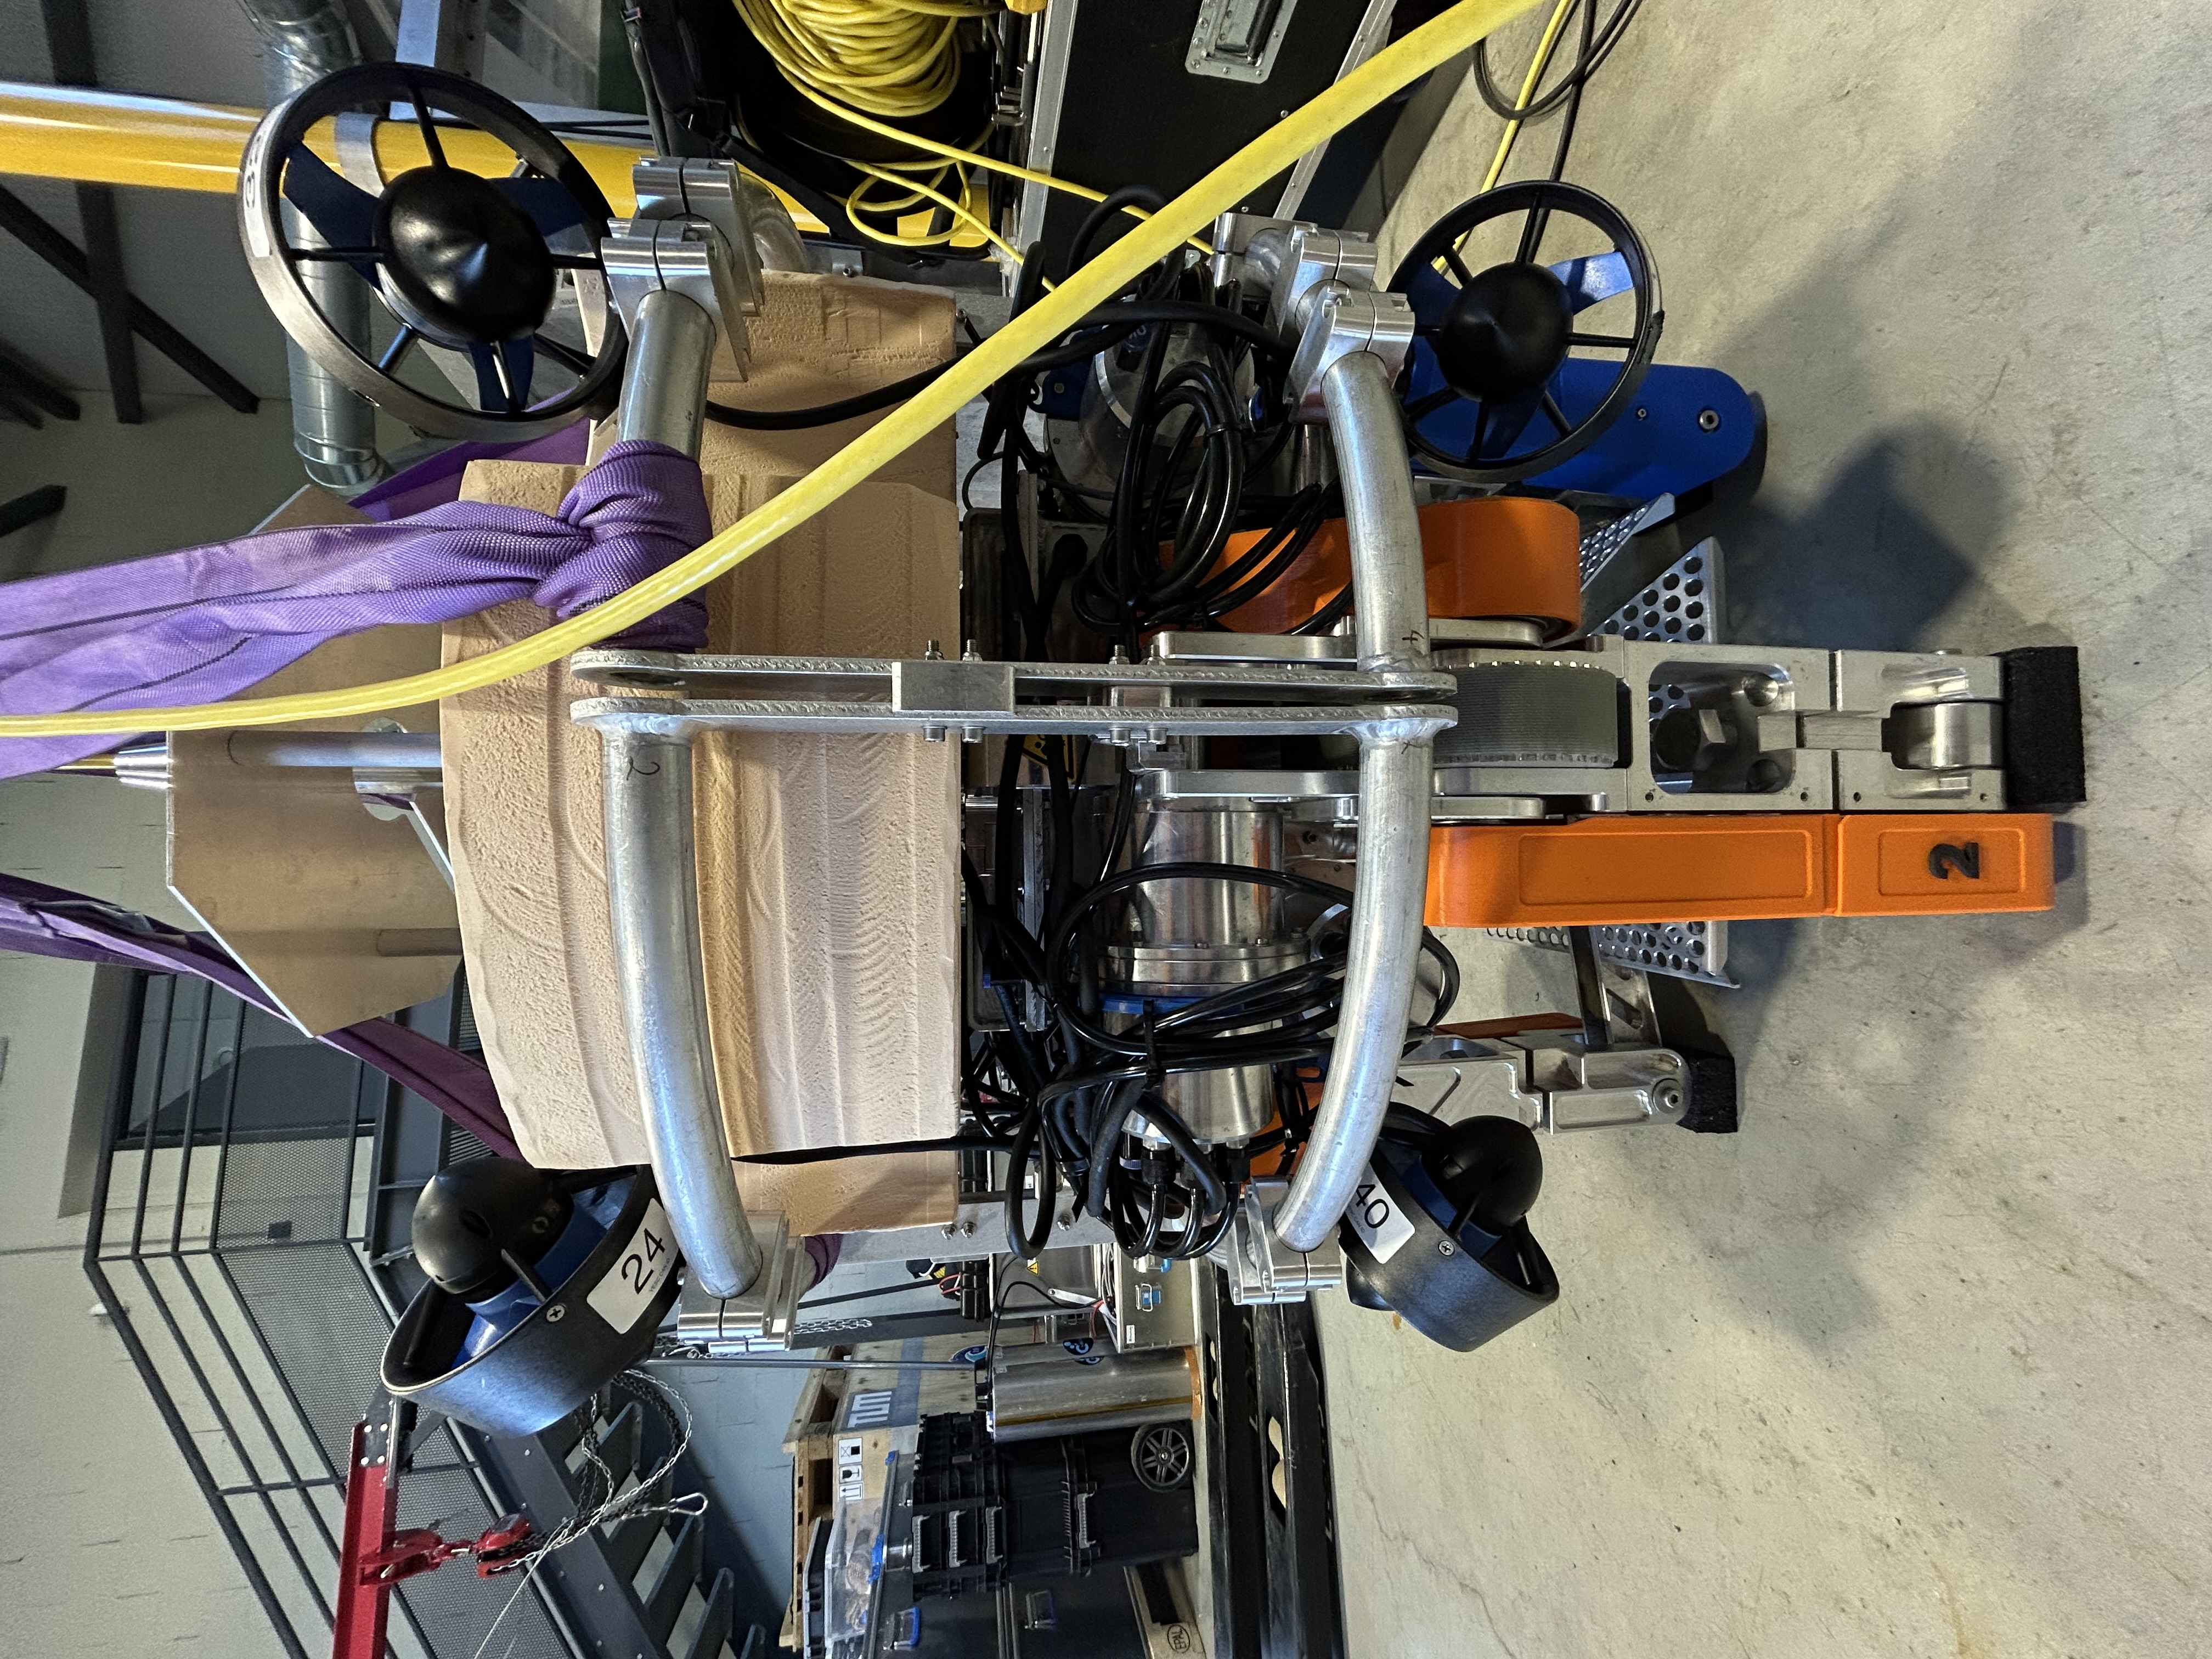
\includegraphics[width=0.25\textwidth, angle=270, origin=c]{img/grapple_thrusters_2.jpeg}\hspace{2pt}%
    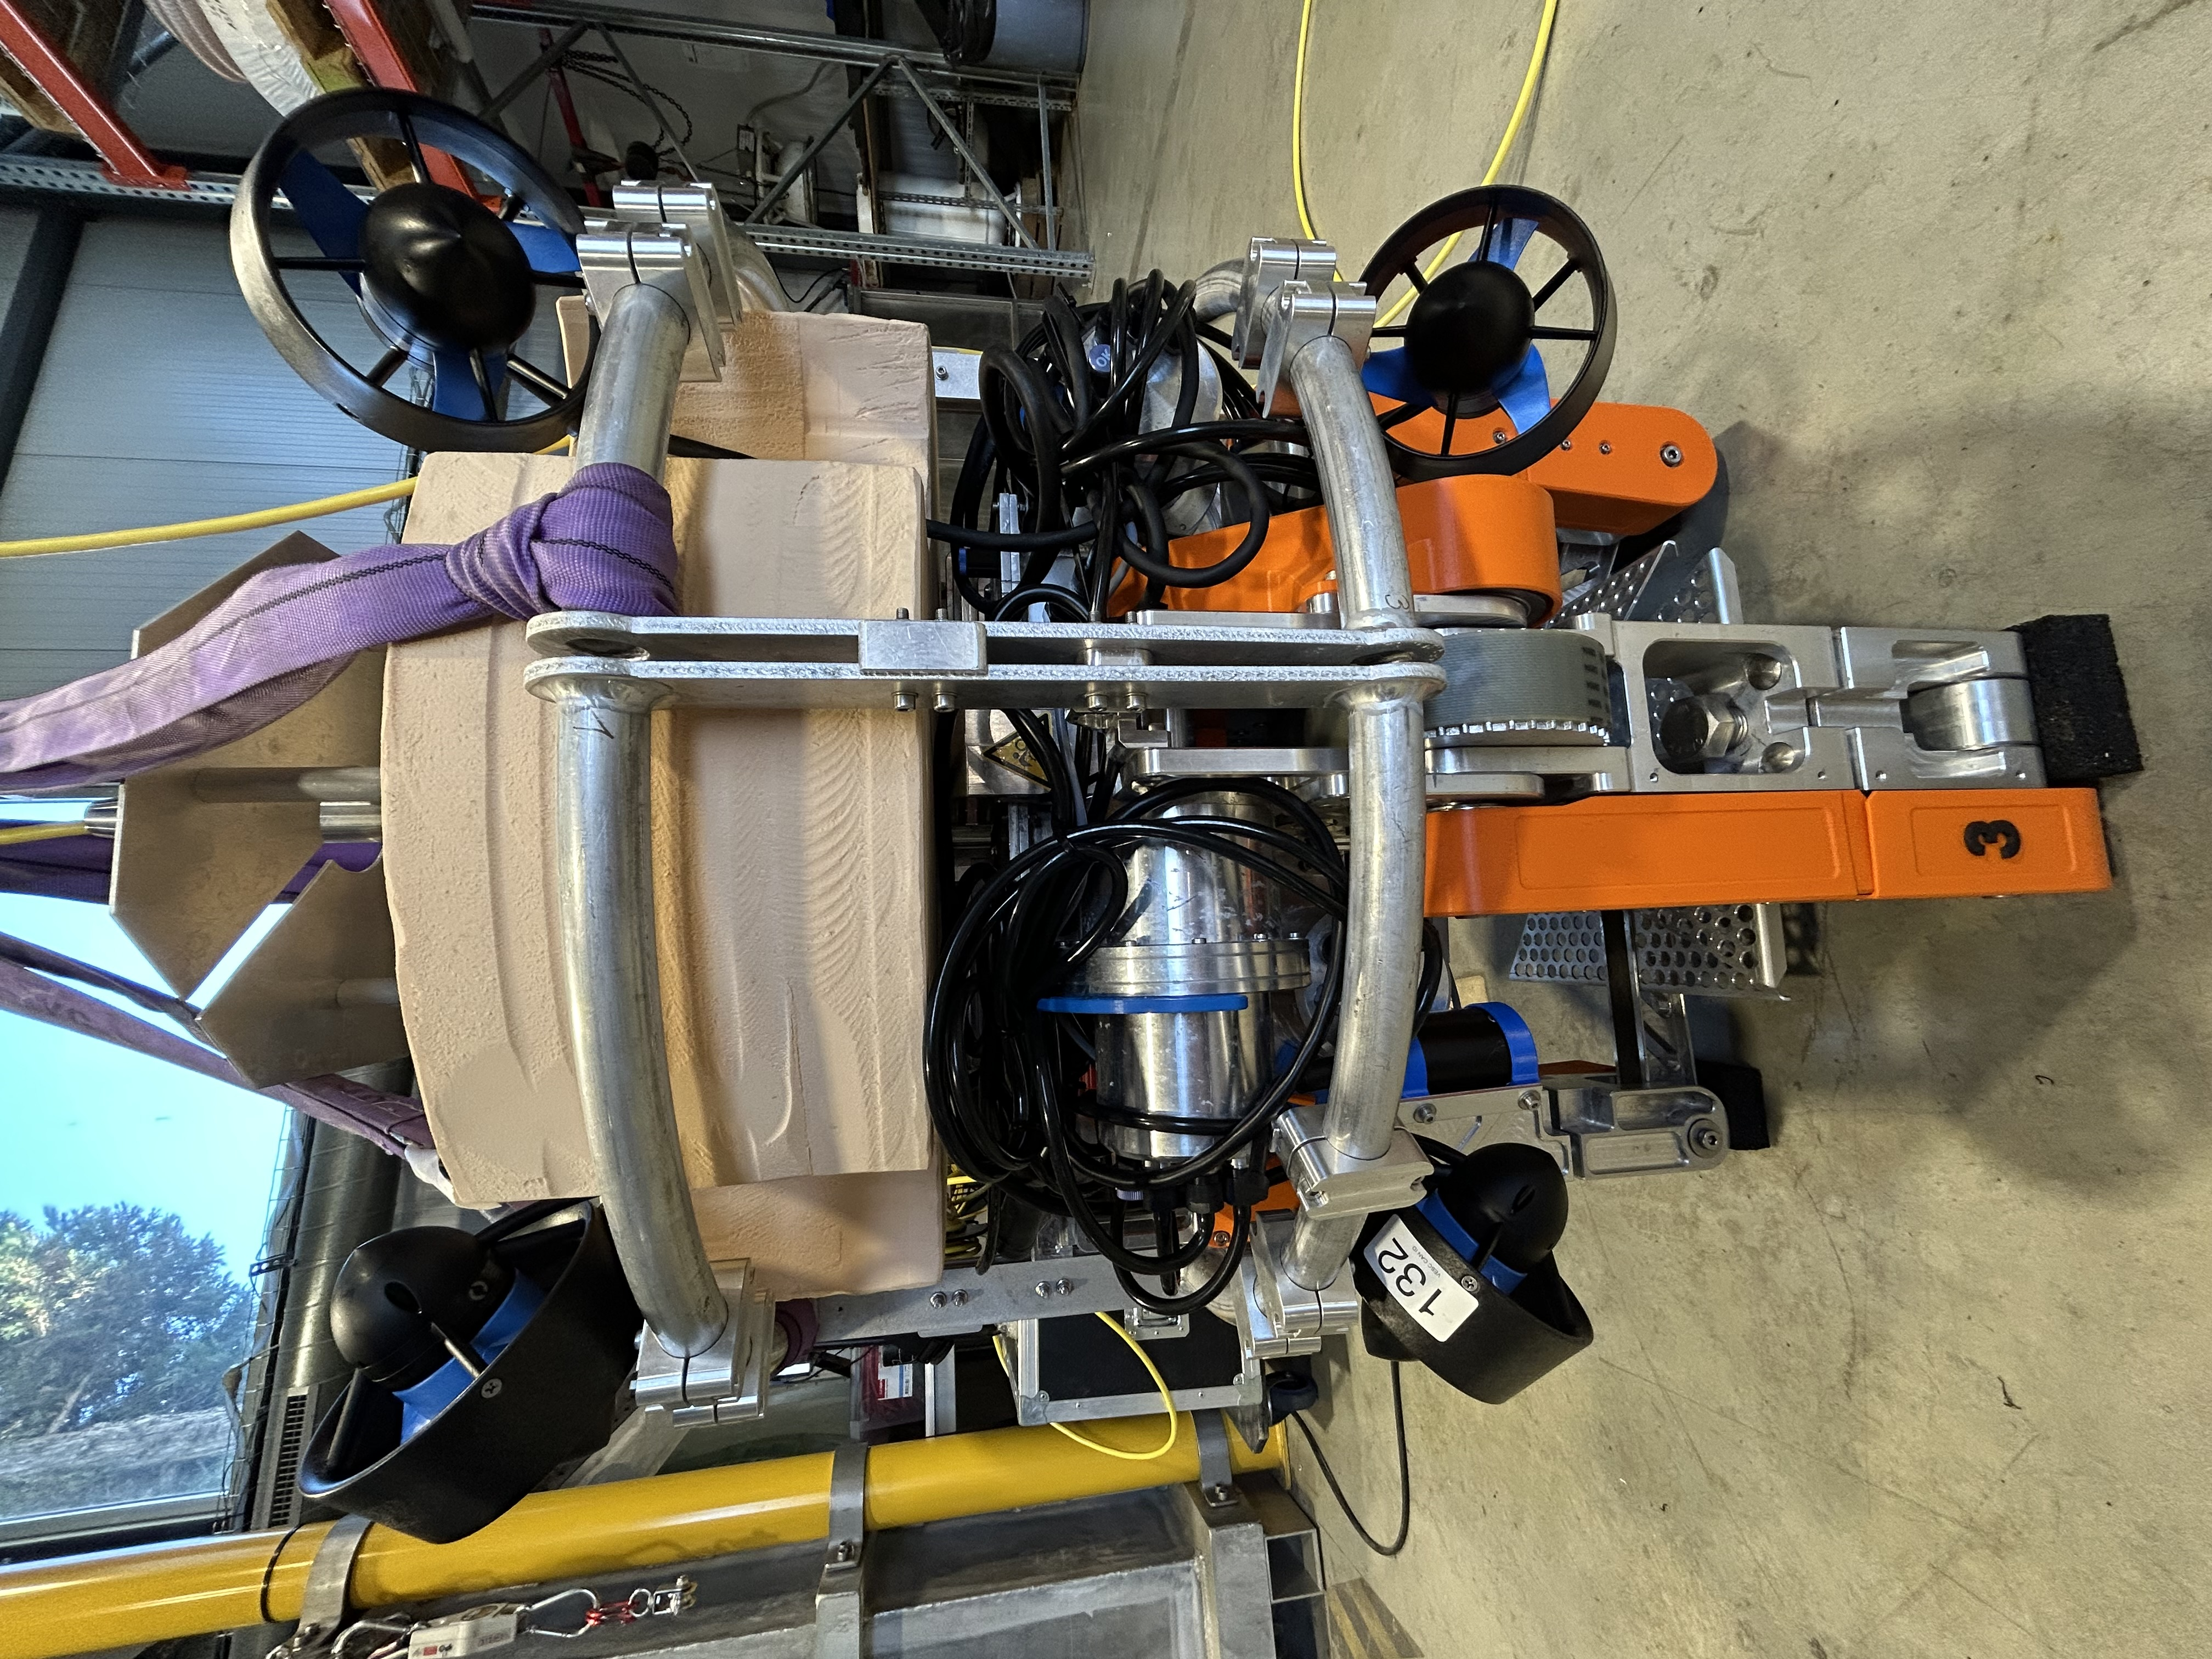
\includegraphics[width=0.25\textwidth, angle=270, origin=c]{img/grapple_thrusters_3.jpeg}\hspace{2pt}%
    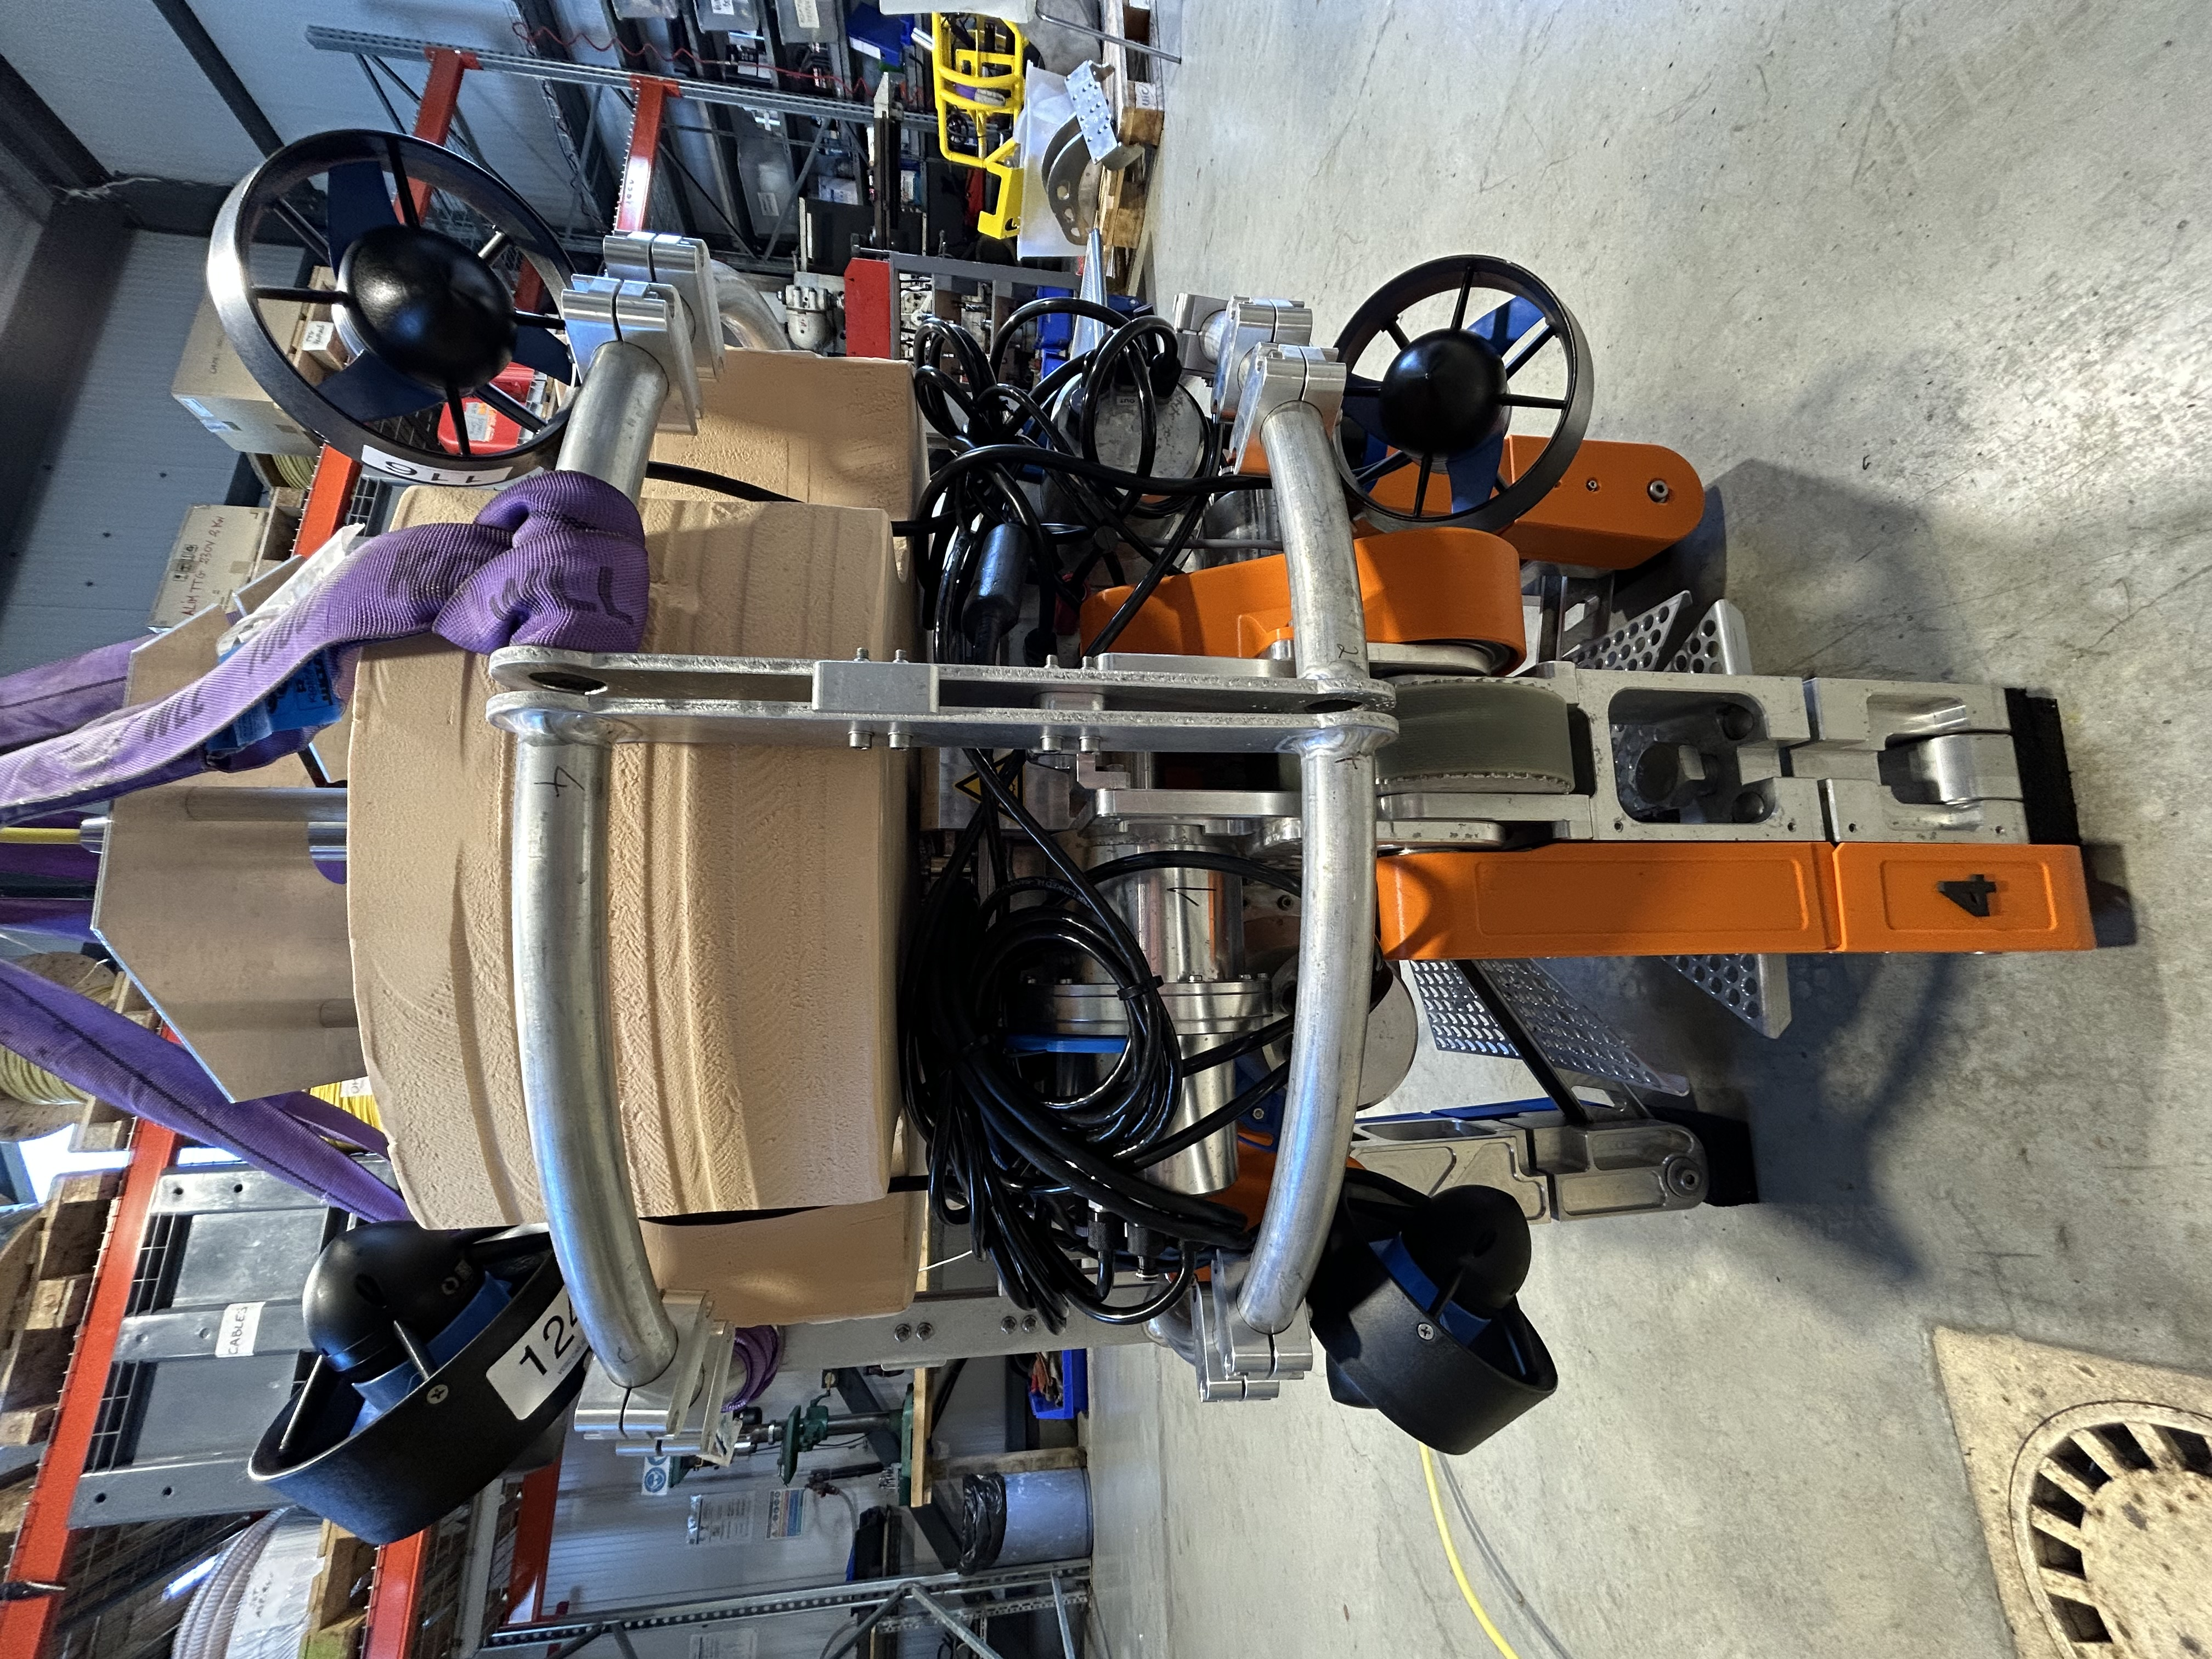
\includegraphics[width=0.25\textwidth, angle=270, origin=c]{img/grapple_thrusters_4.jpeg}\hspace{2pt}%
    \caption{Thrusters layout on the hardware: Marseille (September 2025).}
    \label{fig:thrursters_layout}
\end{figure}

A detailed table on the positions and orientations of the thrusters can be found in Appendix~\ref{appendix:thrustalloc}.


\subsubsection{Derivation of the Control Allocation Matrix}

\bds{Later on 8 is directly used in stead of the general $N$ as on the next line - maybe best link explicitly}
Each thruster \ian{$i \in \{1,\dots,8\}$} is rigidly mounted on the \gls{usg} and defined by its pose with respect to the \gls{usg} reference frame
$\mathcal{F}_{\mathrm{ref}} = (X_{\mathrm{ref}}, Y_{\mathrm{ref}}, Z_{\mathrm{ref}})$.
\paragraph{Position}
Let $\vec{p}_i \in \mathbb{R}^3$ denote the nominal mounting position of thruster $i$ 
expressed in the reference frame $\mathcal{F}_{\mathrm{ref}}$.
Since the allocation matrix is referenced to the \gls{usg}'s \gls{com}, 
located at $\vec{r}_{\mathrm{COM}} = [0, \, 0, \, 0.1362]^\top $, the position vector of thruster $i$ relative to the COM becomes
\begin{align}
\vec{r}_i = R_z(\alpha_0)\,(\vec{p}_i - \vec{r}_{\mathrm{COM}}),
\qquad \alpha_0 = -9^\circ.
\end{align}
because the positions in Table \ref{tab:thruster_pose_nominal_vesc} are expressed \textbf{without }the shift around $Z_{\mathrm{ref}}$ of $\alpha_0 = -9^\circ$, which is seen on Figure \ref{fig:thruster_overview} and in the hardware Figure~\ref{fig:thrursters_layout}. Note that the \gls{com} serves as the reference point for the wrench computation.

\subsection*{Orientation}
Each thruster orientation is defined by the angles
$(\theta_i^{(y)}, \theta_i^{(z)}, \theta_i^{(x)}, \psi_i^{(z)})$.
With
\begin{align}
R_x(\alpha)&=\begin{bmatrix}1&0&0\\0&\cos\alpha&-\sin\alpha\\0&\sin\alpha&\cos\alpha\end{bmatrix}, &
R_y(\alpha)&=\begin{bmatrix}\cos\alpha&0&\sin\alpha\\0&1&0\\-\sin\alpha&0&\cos\alpha\end{bmatrix}, &
R_z(\alpha)&=\begin{bmatrix}\cos\alpha&-\sin\alpha&0\\\sin\alpha&\cos\alpha&0\\0&0&1\end{bmatrix},
\end{align}
the rotation from $\mathcal{F}_i$ to $\mathcal{F}_{\mathrm{ref}}$ is
\begin{align}
R_i = R_z\!\bigl(\psi_i^{(z)}\bigr)
       \bigl(R_x(\theta_i^{(x)})\,R_z(\theta_i^{(z)})\,R_y(\theta_i^{(y)})\bigr).
\end{align}
The inner product of matrices in parentheses represents three consecutive intrinsic rotations, applied successively about the current $y$, $z$, $x$-axes of the thruster. The leading factor $R_z\!\bigl(\psi_i^{(z)}\bigr)$ introduces an additional extrinsic rotation about the fixed $Z_{\mathrm{ref}}$-axis, which represents the shift of $90^\circ$ between consecutive thrusters (Table \ref{tab:thruster_pose_nominal_vesc}).

\paragraph{Homogeneous Transformation} \ian{The transformation matrix with translation and rotation:}
\bds{Best add a sentence or phrase here to aboid a floating equation and to explain what this is}
\begin{align}
{}^{\mathrm{ref}}T_i =
\begin{bmatrix}
R_i & \vec{r}_i\\
\vec{0}^\top & 1
\end{bmatrix}.
\end{align}

\paragraph{Force and Moment Mapping}
Each thruster produces a thrust $u_i$ along its local $+Z_i$-axis:
\begin{align}
\vec{f}_i^{(i)} &= \begin{bmatrix}0\\0\\t_i\end{bmatrix}, &
\vec{f}_i &= R_i\,\vec{f}_i^{(i)} = u_i\,\vec{a}_i,
\quad
\vec{a}_i \coloneqq R_i\!\begin{bmatrix}0\\0\\1\end{bmatrix}.
\end{align}
The resulting moment about the \gls{com} is
\begin{align}
\vec{m}_i = \vec{r}_i \times \vec{f}_i
             = u_i\,(\vec{r}_i \times \vec{a}_i).
\end{align}
The corresponding wrench is
\begin{align}
\vec{\tau}_i =
u_i
\begin{bmatrix}
\vec{a}_i\\
\vec{r}_i \times \vec{a}_i
\end{bmatrix}.
\end{align}
\paragraph{Allocation Matrix}
Stacking all $8$ thrusters gives
\begin{align}
\Mat{B} =
\begin{bmatrix}
\vec{a}_1 & \cdots & \vec{a}_8\\
\vec{r}_1 \times \vec{a}_1 & \cdots & \vec{r}_8 \times \vec{a}_8
\end{bmatrix} \in \mathbb{R}^{6\times 8}, \qquad
\vec{u} = [u_1,\dots,u_8]^\top,
\end{align}
such that
\begin{align}
\boxed{
\vec{\tau} =
\begin{bmatrix}\vec{F}\\\vec{M}\end{bmatrix}
= \Mat{B}\,\vec{u}.
}
\end{align}
\begin{figure}[h!]
    \centering

    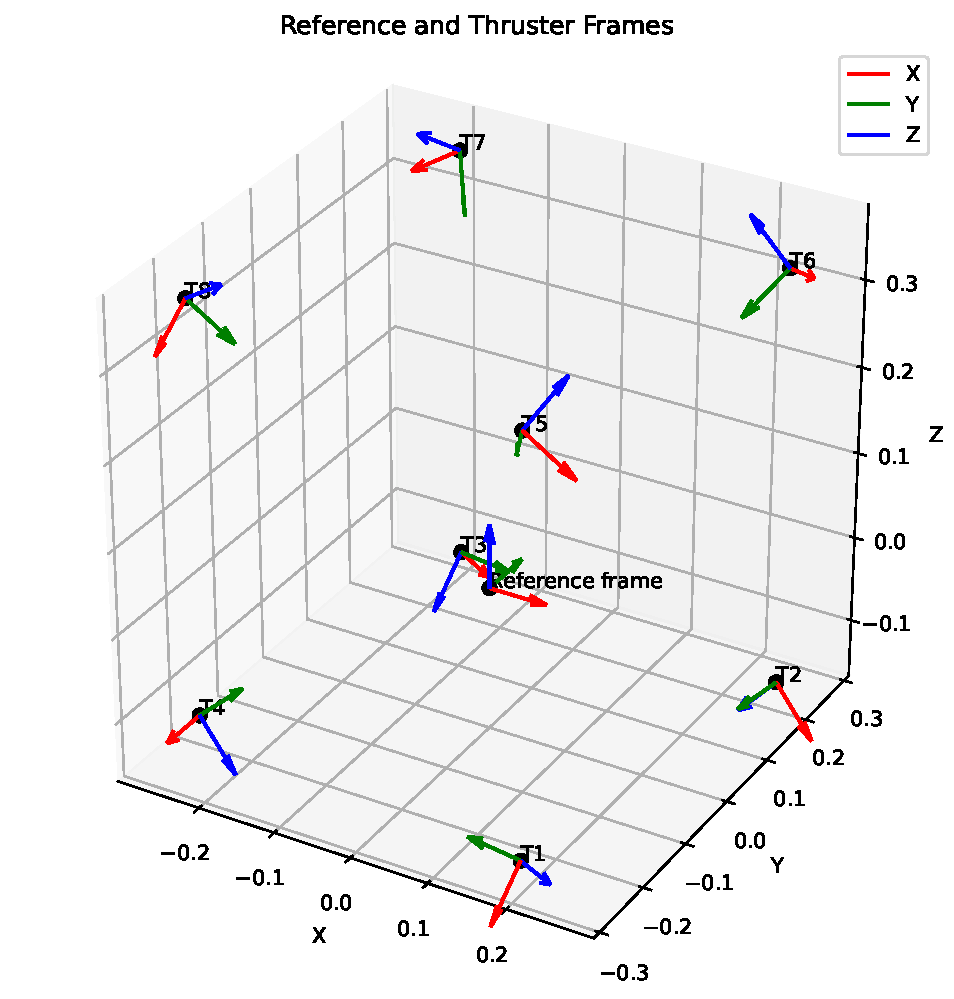
\includegraphics[width=0.28\textwidth, trim={1.5cm 0cm 0cm 0.9cm}, clip]{img/thruster_frames_1.pdf}\hspace{0pt}%
    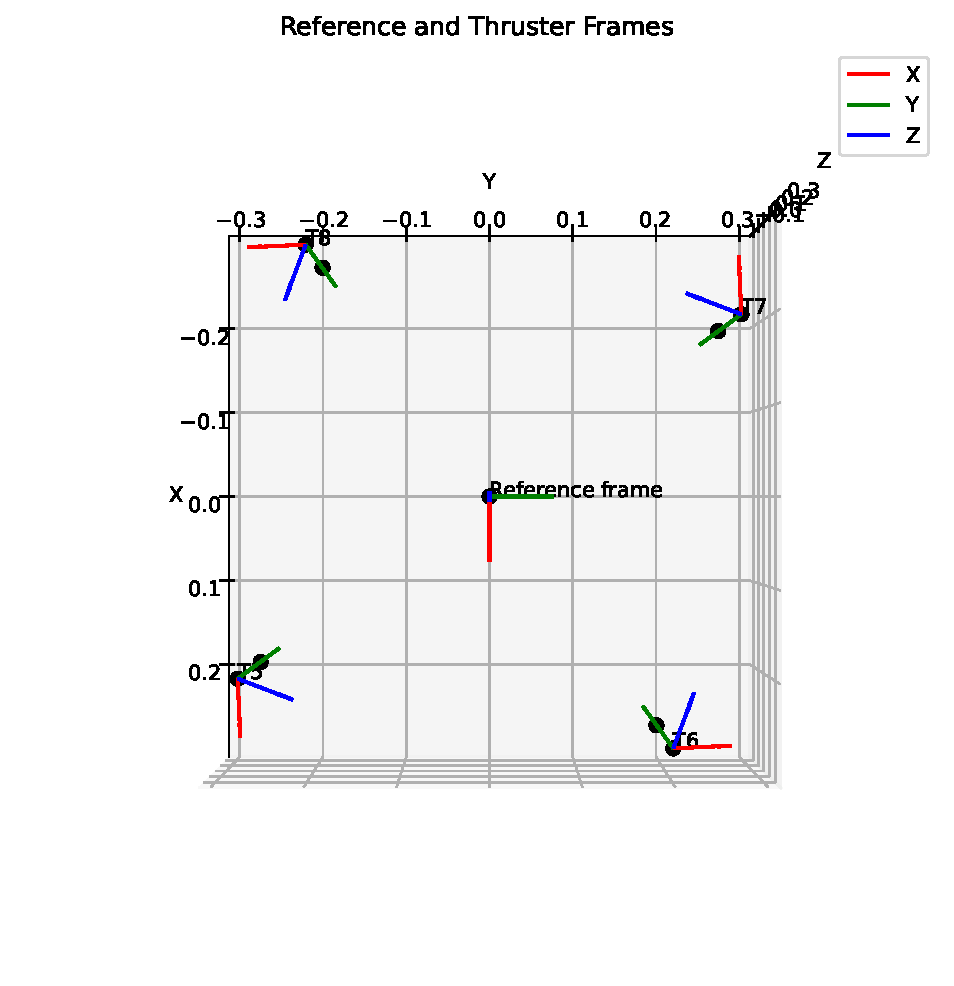
\includegraphics[width=0.37\textwidth, trim={1.5cm 1cm 0cm 0.9cm}, clip]{img/thruster_frames_2.pdf}\hspace{0pt}%
    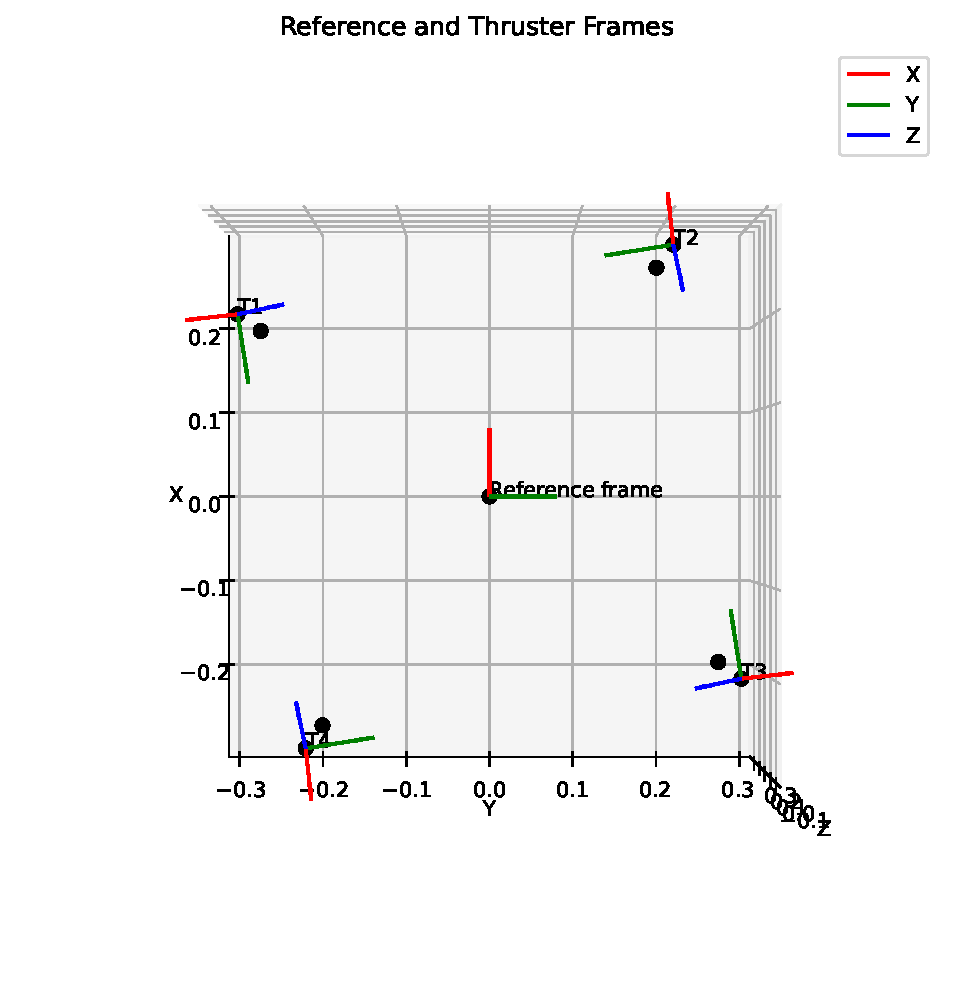
\includegraphics[width=0.35\textwidth, trim={2.5cm 1cm 0cm 0.9cm}, clip]{img/thruster_frames_3.pdf}
        \caption{Thrusters frames obtained after applying the transformations from the reference frame. The blue $Z$-axis also matches the thrust direction.}
            \label{fig:Thrusters_orientations}
\end{figure}

% To ensure the correct configuration, each thruster was labeled with its corresponding VESC motor controllers ID, as specified in the electronics box c.f. Table \ref{tab:thruster_pose_nominal_vesc}.  
For this configuration, the reference frames of the thrusters are illustrated in Figure \ref{fig:Thrusters_orientations}, with IDs according to Table \ref{tab:thruster_pose_nominal_vesc}, where the thrust direction aligns with the local $Z$-axis.


\begin{figure}[htpb]
    \centering
    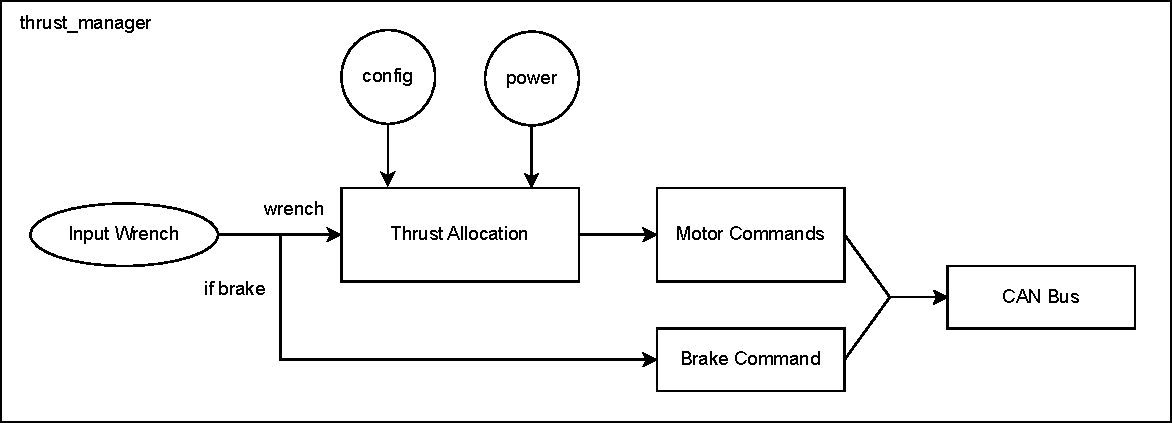
\includegraphics[width=0.9\linewidth]{img/thrust_manager_graph.pdf}
    \caption{Block diagram of \textit{thrust\_manager}}
    \label{fig:thrust_manager_graph}
\end{figure}
\subsubsection{Thruster Allocation Under Power Constraints}
\label{sec:thruster_allocation_power}

This section builds on the approach outlined in Deliverable 3.2. 
Here, we focus on the thrust allocation problem for a given reference wrench. This is a module of the control software referred to as the \textit{thrust\_manager}, see an overview in Figure~\ref{fig:thrust_manager_graph}.

\paragraph{Quadratic Program for Thrust Allocation}

Given a desired reference wrench $\vec{\tau}_{\mathrm{ref}}$, the goal of thrust allocation is to compute the individual thruster inputs $u \in \mathbb{R}^8$ such that the resulting wrench tracks $\vec{\tau}_{\mathrm{ref}}$ as closely as possible while respecting actuator limits. Let $B$ denote the thruster allocation matrix and $W$ a diagonal selection matrix that can deactivate faulty or intentionally disabled thrusters. The nominal allocation problem is formulated as
\begin{subequations}
\label{eq:opt2}
\begin{align}
&\min_{u}\; \frac{1}{2} (BWu - \vec{\tau}_{\mathrm{ref}})^\top H (BWu - \vec{\tau}_{\mathrm{ref}}) 
\label{eq:obj_fun1}\\
\text{subject to} \quad 
& u_{\min} \leq u \leq u_{\max},
\label{eq:ineq_u2}
\end{align}
\end{subequations}
where $H \succ 0$ is a weighting matrix, and $u_{\min}, u_{\max}$ denote the lower and upper thruster bounds, respectively. 
The objective~\eqref{eq:obj_fun1} together with the box constraints~\eqref{eq:ineq_u2} defines a convex \gls{qp}\ian{, e.g., CVXPY}  that can be solved efficiently in real time.\bds{Maybe give some examples of solvers?}



\paragraph{Dynamic Thruster Constraints}
To maintain precise control, ensure that no individual thruster is driven beyond its operational limits, and reduce mechanical wear, the thruster bounds $u_{\min}, u_{\max}$ are adapted dynamically to limit the rate of change of the thruster inputs. 
The bounds are updated based on the previous input $u_{\mathrm{prev}}$ and a maximum allowed rate of change $\triangle u$.

For each thruster $i \in [8]$, \bds{As far as I could see the notation $[n]$ for the set $\{1,2,\dots,n\}$ was not yet defined, unless I overlooked it} \ian{we use $1,2, \cdots,8$} the individual bounds are computed as
\begin{equation}
\begin{aligned}
u_{i,\min} &=
\begin{cases}
    u_{\min} & \text{if } u_{i,\mathrm{prev}} - \triangle u < u_{\min},\\[2pt]
    u_{i,\mathrm{prev}} - \triangle u & \text{otherwise,}
\end{cases} \\
u_{i,\max} &=
\begin{cases}
    u_{\max} & \text{if } u_{i,\mathrm{prev}} + \triangle u > u_{\max},\\[2pt]
    u_{i,\mathrm{prev}} + \triangle u & \text{otherwise.}
\end{cases}
\end{aligned}
\label{eq:maximum_rate_of_change}
\end{equation}
These bounds are defined individually for each thruster and are recomputed at every allocation step. 
In practice, the QP~\eqref{eq:opt2} is solved using the updated bounds $u_{i,\min}$ and $u_{i,\max}$ instead of the static limits $u_{\min}$ and $u_{\max}$.


\paragraph{Available Power and Thruster Power Model}

The smart grapple provides only limited electrical power to the thrusters: the maximum available power is \(P_{\max} = \SI{5}{kW}\), which must be shared between the eight Bluerobotics T500 thrusters and the SensoJoint drives. By contrast, if all eight thrusters operated at their maximum power at \(\SI{24}{V}\), the ROV would require \(8 \times \SI{1044}{W} = \SI{8.35}{kW}\), exceeding the available budget. Hence, the total thruster power must satisfy \(\sum_{i=1}^8 p_i \leq P_{\max}\), where \(p_i\) denotes the power of thruster \(i\).

The mapping between thruster force (or command) and power is nonlinear. For the T500 thrusters, the total power can be approximated as
\[
\sum_{i=1}^8 k_i |u_i|^{3/2} \leq P_{\max},
\]
where \(u_i\) is the control input of thruster \(i\) and \(k_i\) is a fitted constant that depends on whether the thruster operates in forward or reverse mode. Including the power constraint above turns the allocation problem into a nonlinear optimization problem. 
\bds{Insert short sentence to avoid floating equations}
\begin{equation}
\label{eq:NLP}
\tag{\textsc{NLP}}
\begin{aligned}
\min_{u}\;\; &\frac{1}{2} (BWu - \vec{\tau}_{\mathrm{ref}})^\top H (BWu - \vec{\tau}_{\mathrm{ref}}) \\
\text{s.t.}\quad & \sum_{i=1}^8 k_i |u_i|^{3/2} \leq P_{\max}, \\
& u_{\min} \leq u \leq u_{\max}.
\end{aligned}
\end{equation}

To retain the efficiency of a \gls{qp} formulation, we handle the power constraint via a post-processing step, as described below.
\paragraph{Percentage Phase Back (-pp)}
\label{sec:percentage_phase_back}

Since the power constraint in~\eqref{eq:NLP} is nonlinear and incompatible with the \gls{qp} structure, we enforce it in post-processing using a \emph{percentage phase back} strategy~\cite{jenssen2006power}. Let \(u^\star\) be the \gls{qp} solution with total power \(P_{u^\star} = \sum_{i=1}^8 p_i\), and let \(P_{\gls{usg}} \leq P_{\max}\) be the power budget for the thrusters at the time when the optimization is run. If \(P_{u^\star} > P_{\gls{usg}}\), all thruster powers are scaled by
\[
\alpha = \frac{P_{\gls{usg}}}{P_{u^\star}},
\qquad
p_i \leftarrow \alpha\, p_i.
\]
The scaled power of thruster \(i\) is then mapped back to a thrust command \(u_i\) via the fitted T500 power model. For forward and reverse operation this yields
\begin{equation}
u_{i} = \begin{cases}
     \dfrac{-b_{\mathrm{fwd}} + \sqrt{b_{\mathrm{fwd}}^{2} + 4 a_{\mathrm{fwd}} \alpha\, p_{i}}}{2 a_{\mathrm{fwd}}} 
     & \text{(forward)},\\[8pt]
     \dfrac{-b_{\mathrm{rev}} - \sqrt{b_{\mathrm{rev}}^{2} + 4 a_{\mathrm{rev}} \alpha\, p_{i}}}{2 a_{\mathrm{rev}}} 
     & \text{(reverse)},
\end{cases}
\label{eq:percentage_phase_back}
\end{equation}
with \(a_{\mathrm{fwd}}, b_{\mathrm{fwd}}, a_{\mathrm{rev}}, b_{\mathrm{rev}}\) denoting the direction-dependent T500 parameters. This approach allows us to first solve the fast \gls{qp}~\eqref{eq:opt2} without the nonlinear power constraint and then enforce the power limit by a simple scaling and back-transformation, slightly perturbing optimality but preserving real-time feasibility.

To assess the impact of the power constraint and the choice of allocation method, 
we generate a dataset of \(1000\) reference wrenches \(\vec{\tau}_{\mathrm{ref}}\), 
representing desired forces on the \gls{usg}. For illustration, all moments are set to zero,
as the dominant motion is translational. The samples are obtained from a noisy spiral 
path around a sphere. All tests are executed on an Intel(R) Core(TM) i5-6200U 
CPU @ 2.30\,GHz (4 cores), and the thruster power budget is fixed to 
\(P_{\mathrm{thrust}} = \SI{5000}{W}\). We compare the \gls{qp}-pp approach against the 
NLP-based baseline \eqref{eq:NLP} in terms of tracking error~\eqref{eq:obj_fun1} of the desired reference wrench $\vec{\tau}_{\mathrm{ref}}$, power 
consumption, and runtime.

\begin{table}[h!]
\centering
\begin{tabular}{|l|r|r|}
\hline
Approach 
& Error \eqref{eq:obj_fun1} (mean \(\pm\) std.) [\%]
& Power consumption [\%] \\ \hline
\gls{qp}-pp   
& \(+15.6 \pm 11.4\)
& \(+0.2\) \\ \hline
\end{tabular}
\caption{Relative increase in error and average power consumption of \gls{qp}-pp 
compared to the NLP-pow baseline (not shown).}
\label{tab:comparison_power_err}
\end{table}

\begin{table}[h!]
\centering
\begin{tabular}{|l|r|r|r|}
\hline
Approach & Worst case [s] & Avg. runtime [s] & Std. dev. [s] \\ \hline
\gls{qp}-pp    & \textbf{0.0369} & \textbf{0.0181} & \textbf{0.0036} \\ \hline
\eqref{eq:NLP}    & \textit{3.4753} & \textit{0.9000} & \textit{0.4156} \\ \hline
\end{tabular}
\caption{Runtimes for the QP-pp and NLP approaches.}
\label{tab:comparison_power_runtime}
\end{table}

The results \ian{as shown in \cref{tab:comparison_power_err}} \bds{Best refer explicitly to Tables 1 and 2}show that \gls{qp}-pp incurs only a moderate increase in tracking error
(\(+15.6\%\) on average with \(+0.2\%\) higher power consumption) compared to the 
\ian{NLP}\bds{What does "pow" refer to here?} baseline, but achieves roughly two orders of magnitude faster runtimes 
(both on average and in the worst case). Consequently, \gls{qp}-pp is preferred in 
practice, as it enables significantly higher update rates while remaining close to 
the best attainable performance. 

\paragraph{Practical Implementation}
We adopt a modular approach that allows us to overwrite the reference signal at different stages—position, velocity, wrench, or even the duty-cycle command of individual thrusters. This flexibility proved particularly valuable for analyzing and debugging individual modules during the field tests in Marseille (September 2025). The thrusters—and consequently the smart grapple—can be commanded via a \gls{gui}. A position target can be specified (as shown on the left in Figure \ref{fig:thrusters_software}), which is then passed through a cascaded PID controller to generate a target wrench. This wrench is then provided to the optimizer, i.e., the \textit{thrust\_manager} (see Section \ref{sec:thruster_allocation_power}). Alternatively, a velocity command can be set directly—either through the \gls{gui} or using the Logitech gamepad controller—thereby bypassing the position \gls{pid} output. If no \gls{pid} controller is involved, there exists the possibility of providing the reference (to track) wrench directly in the \gls{gui}.

\begin{figure}
    \centering
    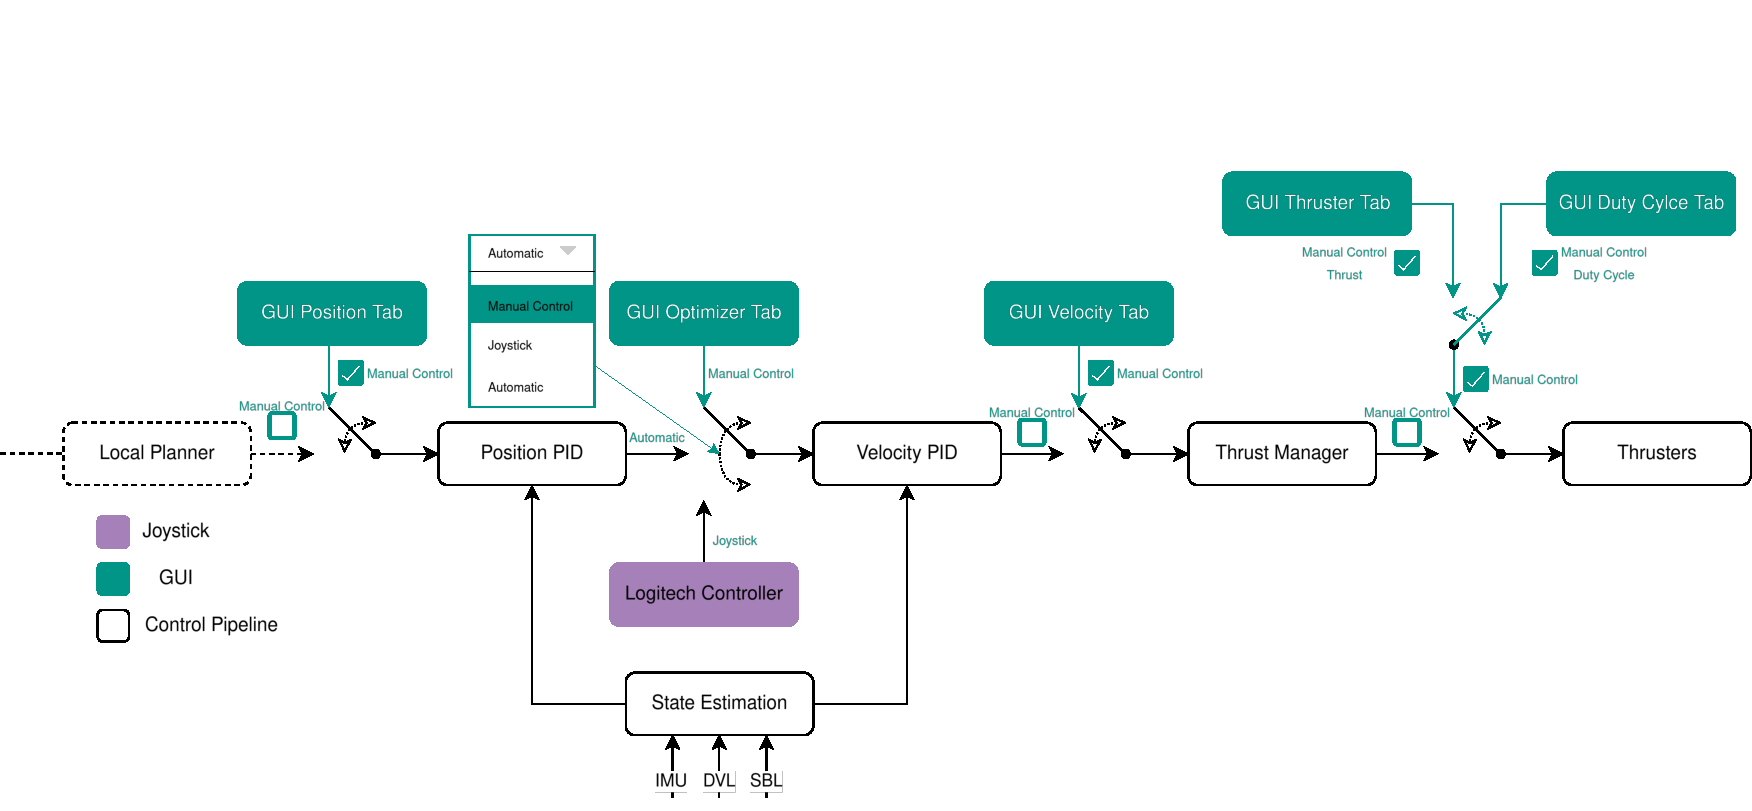
\includegraphics[width=1\linewidth]{img/GUI_documentation.pdf}
    \caption{Architecture of the \gls{usg} control pipeline software.}
    \label{fig:thrusters_software}
\end{figure}

\subsection{Joint control}
The smart grapple joints are actuated by the SensoJoint 5016 BLDC (brushless direct current) motors with a maximal torque of 120 Nm. The motors utilize the \gls{EtherCAT} interface for communication with the computer used for the smart grapple control. In this work, the communication and control of the actuators have been integrated in the overall \gls{ROS2} software architecture using \gls{SOEM} Library \cite{SOEM_library}. All functionalities of the motor can be accessed via a \gls{ROS2} topic or service from any other module of the system. For the convenience of the smart grapple operator, all motor commands can be executed from a \gls{gui} depicted in Figure \ref{fig:sj_gui_screenshot}. 
\subsubsection{Graphic user interface}
The upper button panel contains the ON, OFF, fault reset, and calibration buttons. Pressing ON and OFF will turn the smart grapple on and off, respectively. Turning the smart grapple on means bringing the SensoJoints into the state of enabled operation. From this state, the motors are ready to receive user commands. However, in case of a fault indicated by the built-in fault warning, SensoJoints might enter the fault state, and they will stay in that state unless the fault is cleared by pressing the corresponding button or manually solving the issue onshore. Fault can also be reset automatically by the state machine if it is one of the warnings that can be ignored. The calibration button activates the calibration procedure explained in Section \ref{sec:joint_calibration}.

The lower button panel contains \gls{STO} ON and \gls{STO} OFF buttons. These buttons are connected to the relay inside the electronic box and are responsible for physically connecting and disconnecting the 24V \gls{STO} line. SensoJoint will never be able to reach the operational state without this line connected to the power, as an additional safety measure. \gls{STO} OFF acts as an emergency stop. By default, after the smart grapple has been powered up, the relay is disconnected; therefore, before the operation, the operator is required to press the \gls{STO} ON button.

On the left panel, all the information regarding each joint is displayed, such as the position of the end-effector, velocity, sensed torque, and the fault message. On the central panel, the user has the possibility to control the smart grapple using so-called percentage mode, where \( 0 \%\) corresponds to the fully closed state and \( 100 \%\) to the fully opened state. The joint configuration corresponding to each percentage level is implemented as described in Sec. \ref{sec:percentageControlImplementation}, Case 3. The "Joystick control" checkbox above indicates if the joystick is chosen as the source of input; checking it will disable the slider to avoid conflicting control inputs. The table below the slider displays the joint angles in the smart grapple angle coordinate frame. The smart grapple angle coordinate frame is illustrated in Figure \ref{fig:theta_frame}. \bds{Note that before "Figure" was always put in full, from here in it is being abbreviate; best make this consistent for the entire deliverable} The right panel contains buttons for the relative positioning of the individual joints. By pressing each button, the user opens or closes the joint by 0.05 radians. Using this \gls{gui}, the onshore operator has full monitoring and control over the smart grapple fingers for the manual grasp. 

\begin{figure}
    \centering
    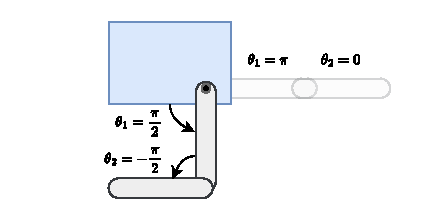
\includegraphics[width=0.6\linewidth]{img/theta_frame_scheme.pdf}
    \caption{Grapple angle coordinate frame.}
    \label{fig:theta_frame}
\end{figure}

\begin{figure}
    \centering
    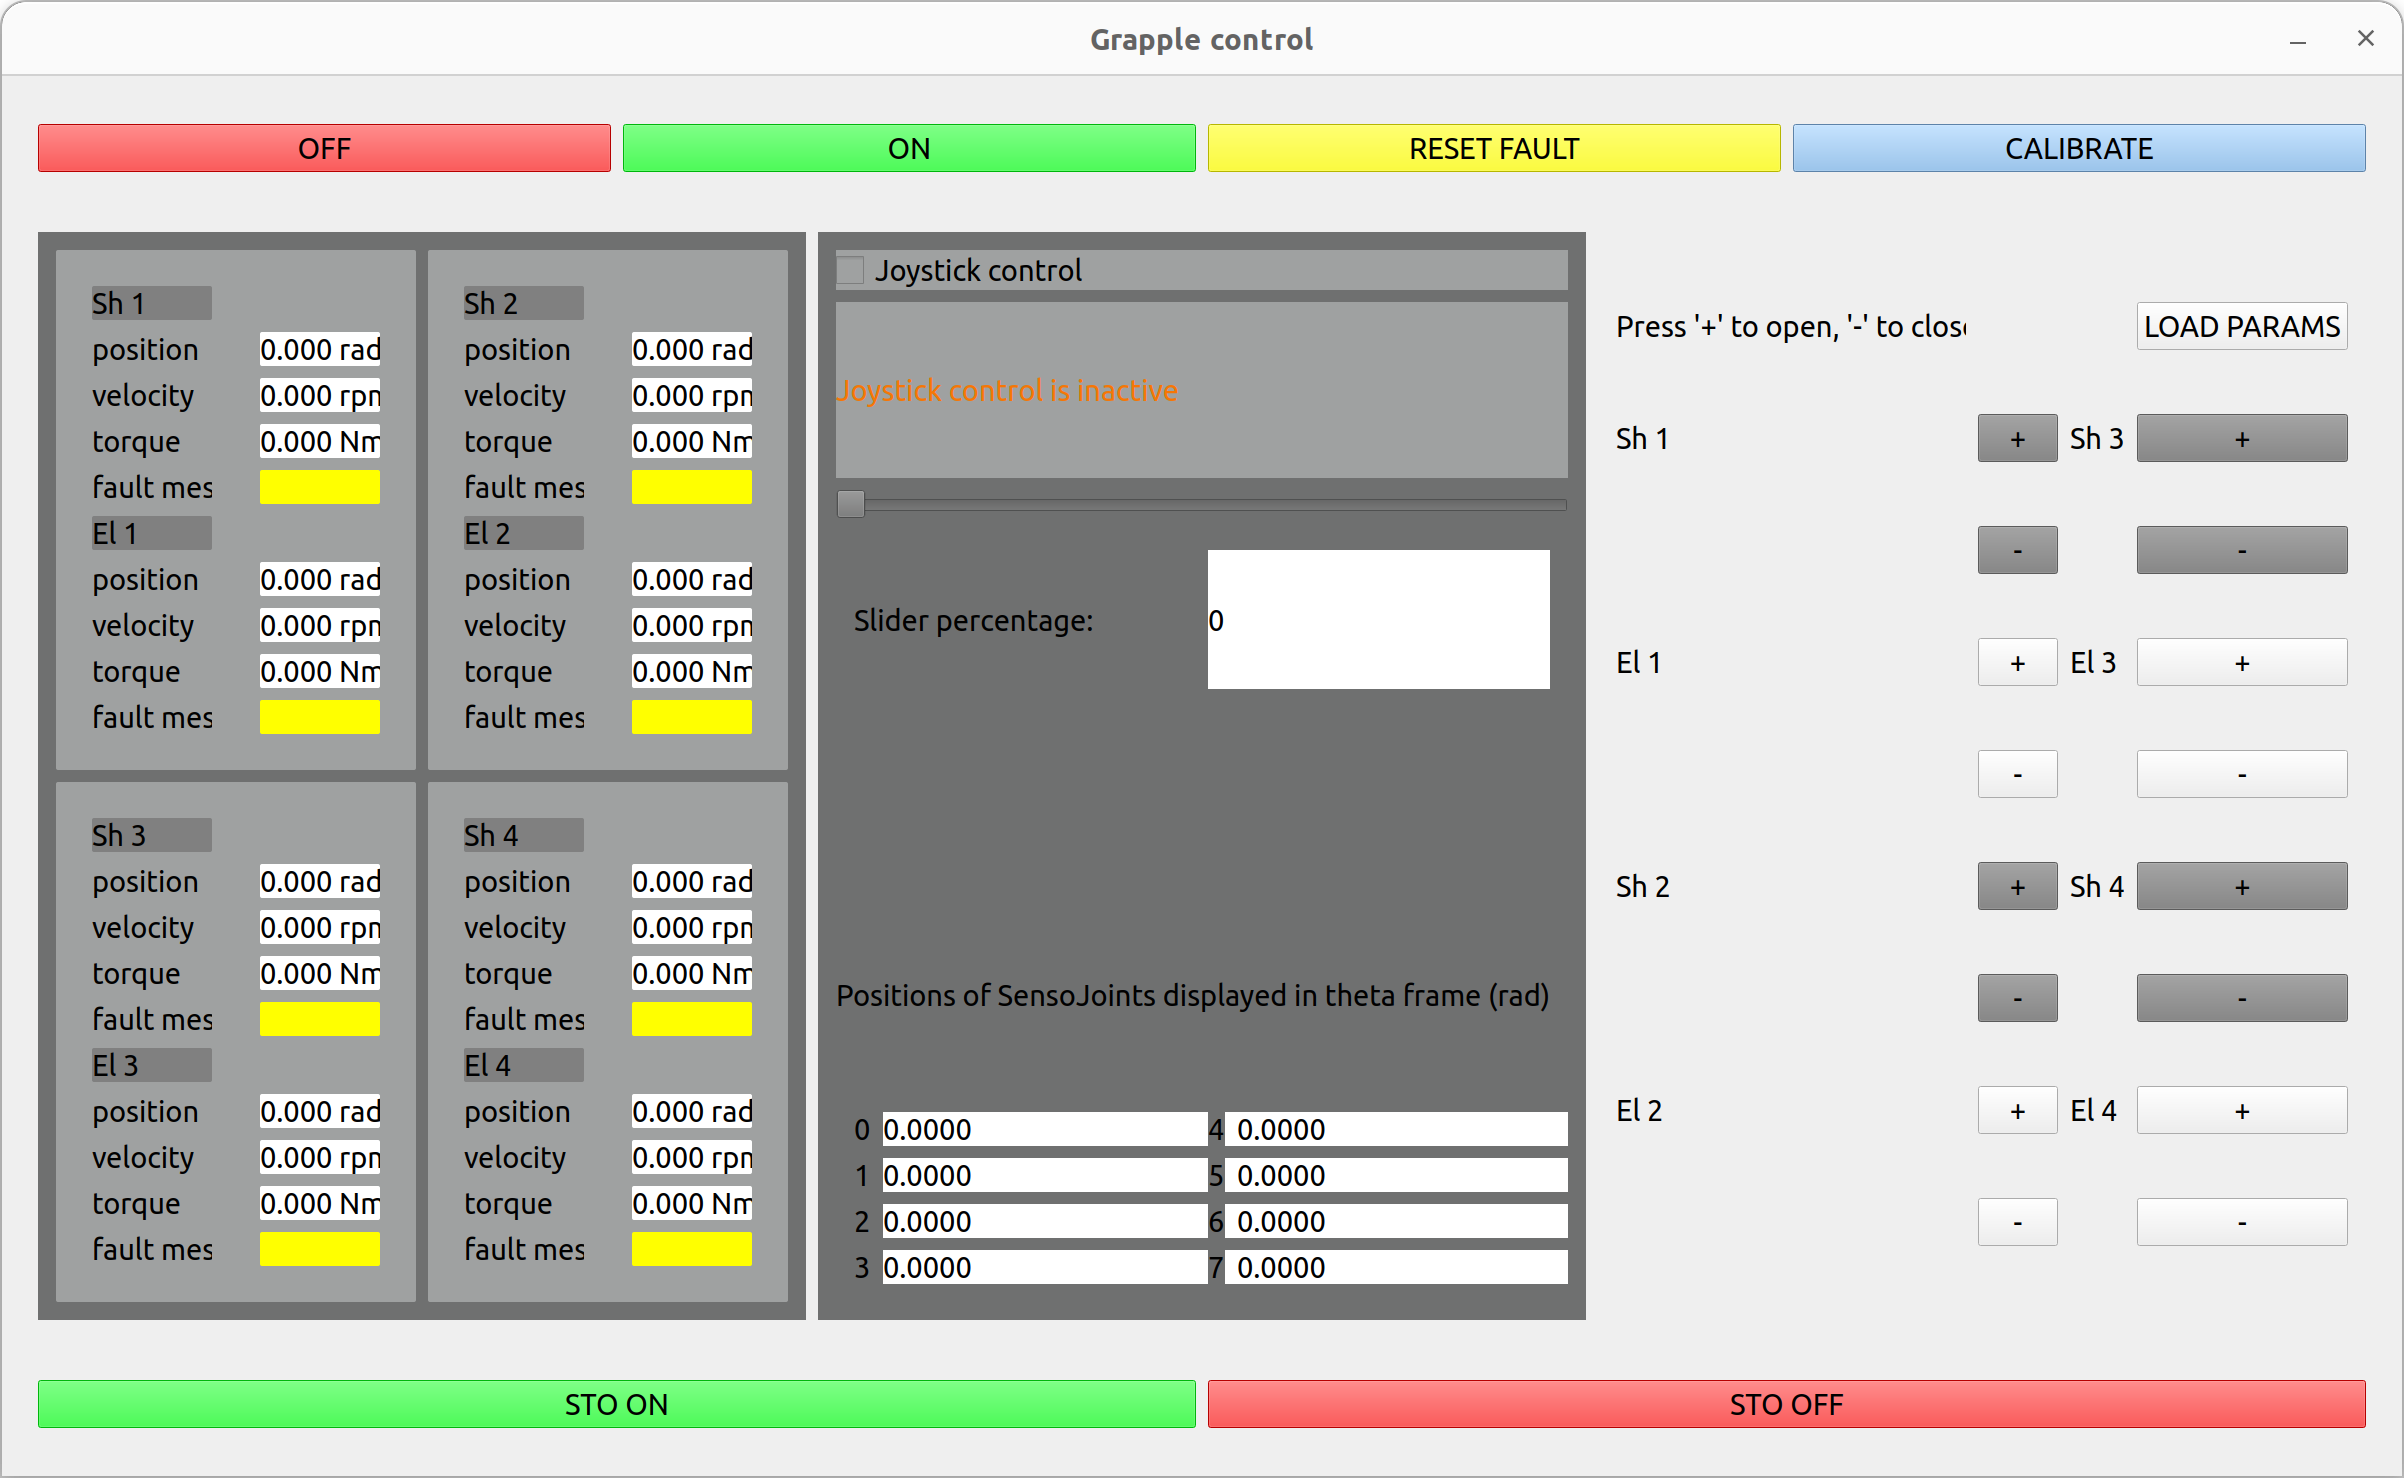
\includegraphics[width=1\linewidth]{img/SJ_GUI_screenshot.png}
    \caption{\gls{gui} for the smart grapple joint control.}
    \label{fig:sj_gui_screenshot}
\end{figure}

\subsubsection{Calibration} \label{sec:joint_calibration}
The calibration routine has been implemented to approximate the angle difference between the encoder zero ("factory zero") and zero in the smart grapple coordinate frame (Figure \ref{fig:theta_frame}). Usually, it must be conducted once, after the smart grapple joint has been reassembled, for example, during routine maintenance. It might also be executed in case of the belt slippage in case of a high joint load. The procedure starts with driving the shoulder joints towards their mechanical limit \bds{remove"above"?} until the predefined torque threshold is reached. Then, the shoulder joints drive back at a small angle to approach the mechanical limit at a lower speed for precision. After that, they are driven on a fixed angle increment between the mechanical limit and the joint angle corresponding to \(\theta_1 = \pi\) in the joint coordinate frame. The same procedure happens then with the elbow joints, but their final position is \(\theta_2 = 0\). After the smart grapple has reached its final starfish-like configuration, the current motor angles are written in the parameter file as \(\Delta\theta_1, \Delta\theta_2\) and later used for angle transformations between encoder angles and smart grapple angles. 

\subsection{State machine of the operation cycle}
The finite state machine is designed to automate the processes of planning, trajectory tracking, precise positioning, grasping, and trash retrieval. The whole cycle of operation is divided into several states, based on the current stage of operation. Transition between states happens in a deterministic manner when particular conditions are fulfilled. The state machine is designed to be responsible for sending activation commands, monitoring the progress, and aborting the operation cycle in case of an error, such as an internal hardware failure. The overall state flow is presented in Figure \ref{fig:general_state_machine}.

\subsubsection{Deploying}
In this state, the initialization procedure happens. The initial storage position of the smart grapple is grasping the collecting net between the SeaCAT \gls{usv} hulls to prevent the unwanted pendulum effect during transportation. Therefore, the deploying state begins with releasing the basket and sending the signal to the SeaCAT \gls{usv} to deploy the grapple under the water. Then, the smart grapple has to be brought into the operational state, which includes a possible joint calibration routine and internal fault check. To be able to transfer to the next state, the smart grapple has to receive the target coordinates as well as the seabed map in the form of an \gls{octomap} \cite{OctomapArticle} from the miniTortuga \gls{uuv}.  
\subsubsection{Planning}
\label{sec:planningState}
As soon as the necessary data are received, no system faults are present, and all components are in the operational state, the smart grapple moves to the planning state. The informed \gls{RRT*} \cite{RRTstarArticle} is currently used in the software to plan a collision-free path, based on the \gls{octomap}, to the first trash object in the received list. Although \gls{RRT*} is used in the current implementation of the control pipeline, it can be replaced by the holistic optimal control approach described in Section \ref{sec:HollisticOptCont}. Once the planning is complete, the state machine activates the tracking state. 

\textbf{Practical implementation} The informed \gls{RRT*} algorithm is implemented using the open-source \gls{ompl} \cite{sucan2012the-open-motion-planning-library}
\subsubsection{Tracking}
\label{sec:trackingState}
The tracking procedure consists of a local planner, state estimation, and the cascaded \gls{pid} controller. The latter then sends the thruster commands according to the architecture illustrated in \ian{Figure} \ref{fig:thrusters_software}. As it is seen from the figure, it is possible to disconnect the direct feedback loop and control the smart grapple using a joystick for debugging purposes. The local planner iterates through the trajectory points provided by the global planner and notifies the state machine as soon as the last one has been reached. Then the tracking state is considered as finished. It is possible that, due to the environmental conditions, such as strong tides, the smart grapple will not position itself directly above the target. In this case, a precise positioning procedure is required to reposition the grapple for the grasp. The next state depends on two factors: whether the user wants to proceed with the manual grasp and whether the visual servoing is feasible. During the development process, the manual grasp is selected, and the smart grapple is navigated solely by the operator onshore using the joystick and the \gls{gui} to control the fingers. The availability of the visual servoing depends on the visibility conditions of the environment. In case of good visibility, the  smart grapple makes a state transition to the visual servoing state, described below. In case of bad visibility, the smart grapple has to position itself based on the last known position of the trash. 

\subsubsection{Visual servoing}
The visual servoing state has the purpose of camera-driven, precise position control of the smart grapple. \bds{it's not clear here when does the visual servoing start and when does the path planning phase stops. Also, how is the reference position expressed for visual servoing compared from the earlier path planning phase. Figure 11 could be linked here?}
\revision{This state is triggered upon reaching the final path point, provided that water clarity is sufficient for object detection. In this phase, the reference position for the controller is expressed in the camera-based coordinate frame. (Figure \ref{fig:general_state_machine}).
Specifically, the object detection model (Section 4.1) identifies the target and provides its bounding box coordinates, while the optimal grasp point estimation algorithm (Section 5.4) determines the desired grasp pose.
The control objective is to center the bounding box within the onboard camera's horizontal frame and reach the desired altitude (pose) vertically using the \gls{dvl} \bds{Use abbreviation LateX package here too} feedback.
Once the desired pose is achieved, the state machine transitions to the grasping state.}

\subsubsection{Grasping}
\textbf{Automated grasp}
The automated grasping state consists of its own state machine illustrated in Figure \ref{fig:alg_torque_monitor}. The general state machine is responsible for initiating the grasping procedure by calling a corresponding \gls{ROS2} service and passing the desired contact points for the grasp from the algorithm described in Section \ref{sec:Gripping_points_opt} (if available). During the automated grasp, it is possible that the actuators activate the built-in maximum torque warning and enter a fault state. In this case, the state machine is responsible for sending the fault-clearing signal unless the fault cannot be cleared automatically (e.g., a finger has to be manually opened to release the torque), and the smart grapple must be switched to manual control. 

\textbf{Manual grasp}
The manual grasp is controlled using the \gls{gui} illustrated in Figure\ref{fig:sj_gui_screenshot}. For the manual grasp to be considered as completed, the user has to initiate the state transition from grasping to dropping by calling a corresponding \gls{ROS2} service.

In case of a successful grasp, the state transitions to the dropping (recovering) state.

\subsubsection{Dropping (Recovering)}
In the dropping state, the state machine sends the signal to the \gls{usv} Tender (illustrated in Figure \ref{fig:SC2concept }), initiating the retrieval of the object grasped. The smart grapple sends the signal to roll the tether, positioning itself above the water, and waits for the \gls{usv} Tender to position itself below. After receiving the signal, approving the object drop, it opens and measures the joint torques. It might happen that due to the seaweed and sediment, the object or parts of it get stuck in the shovels or on the joints. If the excess torque is sensed, the smart grapple will try to repeat the cycle of opening and closing \ian{\(k\)} times \bds{Note that before N was the number of thrusters}, before reporting an error due to the impossibility to continue its operation. The number of tries \(k\) is a system parameter that can be set by a user. After the successful dropping, the smart grapple can proceed with the next object in the list, or the operator can declare the operation finished, and the smart grapple will send a signal to the SeaCAT \gls{usv} to be brought back to shore.

\subsubsection{Error}
The error state is activated in case of an error in any state of operation. The error state means that the state machine notifies the onshore operator about its inability to continue the cycle, and the SeaCAT \gls{usv} brings the smart grapple back to the shore for maintenance. The possible errors include 
\begin{enumerate}
    \item SensoJoint faults that cannot be resolved automatically
    \item Thruster communication failure
    \item Object being stuck in the shovels or in the joints
    \item User-defined error, when the error state is activated by the operator
\end{enumerate}
\begin{figure}
    \centering
    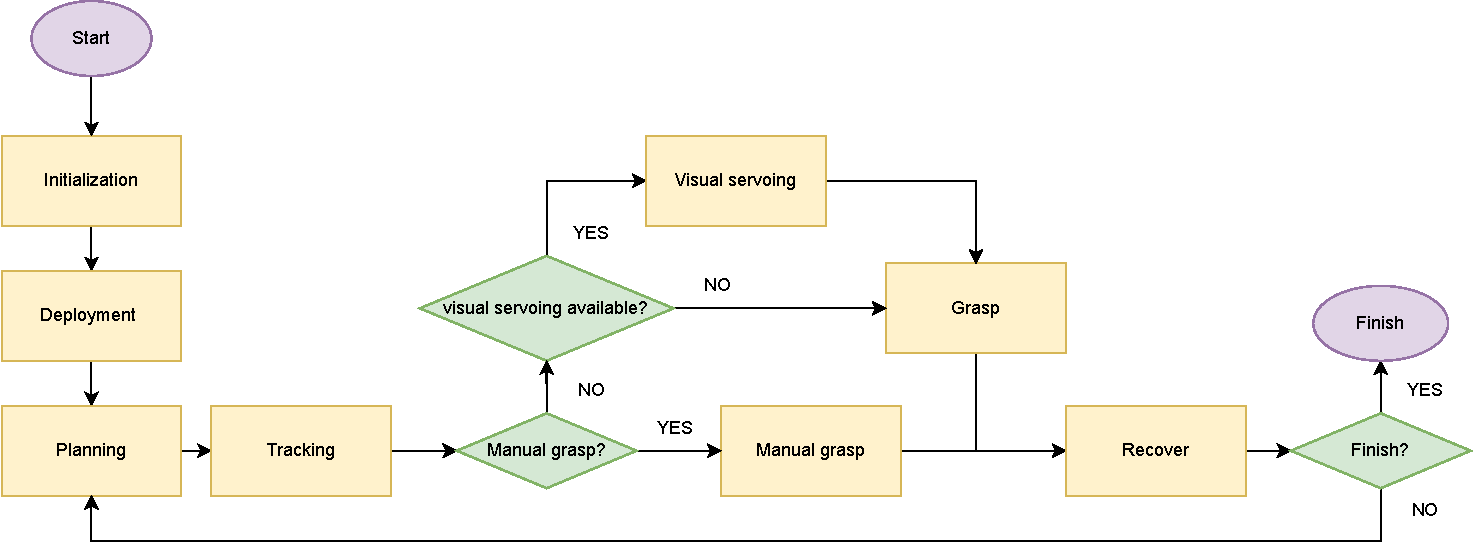
\includegraphics[width=1\linewidth]{img/overall_state_machine.drawio.pdf}
    \caption{Operation state flow.}
    \label{fig:general_state_machine}
\end{figure}
